\documentclass[letterpaper,twocolumn,10pt]{article}

%usenix/complementary_newdefines.cls

\usepackage{usenix,epsfig,endnotes}

%\documentclass[times, 10pt, twocolumn]{article}
\usepackage{amssymb} %for \varnothing
\usepackage{times}
\usepackage{amsfonts}
%\usepackage{amsthm}

\usepackage{float}
\usepackage{graphicx, multirow}
\usepackage{amsmath}

\usepackage{listings}
\usepackage{url}
\usepackage{mathtools}
\usepackage{amssymb}
\usepackage{cite}

\usepackage[colorlinks=true,linkcolor=black,citecolor=black,urlcolor=black]{hyperref}
%customized packages

\newtheorem{theorem}{Theorem}[section]
\newtheorem{lemma}[theorem]{Lemma}
\newtheorem{proposition}[theorem]{Proposition}
\newtheorem{corollary}[theorem]{Corollary}

\newenvironment{proof}[1][Proof]{\begin{trivlist}
\item[\hskip \labelsep {\bfseries #1}]}{\end{trivlist}}
\newenvironment{definition}[1][Definition]{\begin{trivlist}
\item[\hskip \labelsep {\bfseries #1}]}{\end{trivlist}}
\newenvironment{example}[1][Example]{\begin{trivlist}
\item[\hskip \labelsep {\bfseries #1}]}{\end{trivlist}}
\newenvironment{remark}[1][Remark]{\begin{trivlist}
\item[\hskip \labelsep {\bfseries #1}]}{\end{trivlist}}

\newcommand{\qed}{\nobreak \ifvmode \relax \else
      \ifdim\lastskip<1.5em \hskip-\lastskip
      \hskip1.5em plus0em minus0.5em \fi \nobreak
      \vrule height0.75em width0.5em depth0.25em\fi}

\pagestyle{empty}

\DeclarePairedDelimiter{\ceil}{\lceil}{\rceil}
\let\oldemptyset\emptyset
\let\emptyset\varnothing

\newcommand\defeq{\stackrel{\mathclap{\normalfont\mbox{def}}}{=}}
\newcommand{\overbar}[1]{\mkern1.5mu\overline{\mkern-1.5mu#1\mkern-1.5mu}\mkern 1.5mu}

\DeclareMathAlphabet{\mathcal}{OMS}{cmsy}{m}{n}

\sloppy

\begin{document}

\title{On the security of encryption and compression composition}

\author{
    Anonymized submission
}
%  \author{
%      \rm Dimitris Karakostas \\
%      University of Athens \\
%      dimit.karakostas@gmail.com
%      \and
%      Aggelos Kiayias \\
%      University of Edinburgh \\
%      akiayias@inf.ed.ac.uk
%      \and
%      Dionysis Zindros \\
%      University of Athens \\
%      dionyziz@di.uoa.gr
%  }

\maketitle

% Use the following at camera-ready time to suppress page numbers.
% Comment it out when you first submit the paper for review.
\thispagestyle{empty}

\begin{abstract} When compression is composed with encryption, unexpected
vulnerabilities can arise. Such vulnerabilities have been explored in practical
attacks against TLS such as CRIME, TIME, and BREACH, even after TLS 1.3.
Motivated by the lack of production-grade testing tools, we provide Rupture, a
modular scalable open-source generic attack framework that implements
compression side-channel attacks in a robust manner. We introduce an abstract
theoretical cryptographic model to express such attacks, the \textit{adaptive
reflection security} game with the relevant security definitions. We propose a
model for \textit{compression idealness} and experimentally show that typical
compression functions expose partially ideal behavior. We then argue that
typical plaintexts used in practice follow an interdependent joint distribution,
a stronger notion of dependent joint distributions. Based on these two
properties, we prove that \textit{compression-detectability} of predicates
arises, i.e. the ability to extract a predicate of the plaintext using
reflection. We then prove that all length-preserving encryption schemes are
insecure when composed with such functions.  Finally, we propose a novel defense
protocol, \textit{context hiding}, that effectively eliminates the threat these
attacks pose. This protocol modifies the plaintext joint distribution in order
to remove the interdependence and mitigate the problem.  We argue about the
security of our defense method. We show that our method of defense performs
significantly more favourably in terms of compression rate compared to previous
techniques.\end{abstract}

\section{Introduction}\label{sec:prev}

Compression and encryption composition has caused serious security problems in
protocols such as TLS \cite{dierks2008tls} over the years with an array of
attacks making major headlines in computer security dissemination forums,
including BREACH \cite{gluck2013breach}, TIME \cite{be2013perfect}, and CRIME
\cite{duong2012crime}. Although the idea that compression is a side-channel that
can be exploited is certainly folklore in the cryptography community and is
documented at least as early as Kelsey's work \cite{kelsey2002compression}, a
proper theoretical model capturing the real-world perspective of these
side-channel attacks is still elusive.

Motivated by this, in this paper we introduce a general model that incorporates
the rendering process that is exploited during these attacks and facilitate a
thorough theoretical analysis of the security of encryption-compression
composition. We showcase the power of our approach by (i) demonstrating an
improved attack framework, called Rupture, that improves substantially the
performance of previous attacks, (ii) showing how attacks like BREACH
\cite{gluck2013breach}, TIME \cite{be2013perfect}, and CRIME
\cite{duong2012crime}, can be expressed as instances of our compression
side-channel attack template, (iii) presenting a general mitigation strategy,
called CTX, that strikes a good balance between security and efficiency and can
be readily incorporated in a TLS deployment without a significant performance
degradation.

\subsection{Contributions}
Our contributions are as follows.

First we introduce a novel model for analyzing compression and encryption
composition attacks, the \textit{adaptive reflection game}, with an accompanying
security definition. This model is quite general in that it does not describe
specific instances of the rendering function $f$ or the compression function
$\textrm{Com}$. Furthermore, it allows for general distributions of secret $\mathcal{M}$
and distributions of noise $\mathcal{V}$ which can affect the rendering. Section
\ref{sec:refsec} contains the definition of this model.

We wish to prove that all encryption functions are insecure when composed with
compression. In order to produce this proof, we build a series of required
assumptions.

We define \textit{interdependence}, a property that characterizes dependent
random variables drawn from a joint distribution. Interdependence is an
important notion when exploring the effects of the reflection when compressed
with a secret. We introduce interdependence in section
\ref{subsec:interdependence}.

Another property of compression functions is \textit{compression idealness} with
respect to a message distribution. We
define idealness in theory and demonstrate how it applies on the compression
algorithms that are widely used in section \ref{subsec:com_idealness}.

Based on the properties of compression idealness and interdependence, we prove
that predicates on the secrets can be learned by choosing adversarial
reflections. We call this property \textit{compression detectability}, which we
explore in section \ref{sec:propertycom}.

The final part of our theoretical work on the attack is to show that this
somewhat innocent property directly allows the construction of an attacker,
which we prove breaks the security of the scheme in section
\ref{sec:comattack}. We also prove that such attacks can be amplified to
achieve better confidence.

At this point we implement Rupture\footnotemark[1], a production-grade open
source framework for conducting compression and encryption composition attacks.
This generic framework provides an extensible mechanism for experimentally
testing attack techniques in a modular setting. We implement specific
compression attack instances such as BREACH. This is the first time a working
tool is provided for this class of attacks.  Based on our attack framework we
achieve significant improvements in our implementation compared to previous
attempts. We improve the complexity from linear to logarithmic in the secret
alphabet's size, we attack block ciphers in addition to stream ciphers and we
employ practical techniques for network level optimization.  Rupture is further
described in section \ref{subsec:rupture}.

Having established the attack premises, we shift our interest in defending
against such attacks. Although there are several proposed defenses, we feel that
none achieves good compression performance in real-world system terms. In this
direction, we propose \textit{context hiding}, a method that mitigates a class
of practical compression side-channel attacks like BREACH. Context hiding aims
at preventing the compression detectability of a predicate $Q$ of a secret $s$
in presense of reflection as described in section \ref{sec:defense}.

Our implementation of the context hiding defense technique is called
CTX\footnote[1]{The GitHub repositories of the Rupture and CTX projects make the
source code openly available but have been removed for anonymization purposes
and can be provided upon request.}. CTX runs at the application layer of web
services and is opt-in. It is implemented in Python and Javascript and can be
used in the common web frameworks Django, Flask and Node.js. CTX achieves
balance between security and compression performance that is unprecedented
compared to other proposed defense methods.

We experimentally show in section \ref{subsubsec:ctx_experiments} that CTX
performs well in terms of size and time overhead. Specifically, we find that the
performance penalty of CTX compared to other proposed methods, like secret
masking, is significantly lower and within accepted rates for real-world
applications.

\section{The attack}\label{sec:attack}

\subsection{A high-level overview}\label{subsec:example}
As explained above,  compression side-channel attacks pose a serious threat
against real-world deployments of TLS and in general of
any encryption system. While widely received and documented
by the security community there are still not many mitigation strategies in place
to thwart them, primarily due to (i) the perceived high performance
penalty associated with mitigating them, and
(ii) their perceived complexity and
the lack of production code tools
that allow for their robust execution, something that makes some believe
they are not a realistic threat. In this work we will illustrate that
these perceptions  are wrong
and the existence of these attacks
suggests  a grave situation that is critical to be addressed.

In order to appreciate the seriousness of these attacks we present a motivating
example.
Suppose that  a  user that browses the Internet and a server
that hosts a website are in active communication.
This website might be a social network, e-banking, mail
provider or a similar service that handles sensitive private data. When the
server receives a request for a web page it collects all needed data, generates
the HTML code that will be displayed by the user's browser and sends a network
response containing this code along with other resources such as images and
libraries. All response data is encrypted under TLS, which ensures privacy and
integrity for the communication between the user and the server,
but also compressed for efficiency.

Consider now an adversary that aims to break this communication's security.
This adversary tries to decrypt the communication between
the user and the server and reveal information about the private data that is
exchanged. In order to mount a compression side-channel attack certain
conditions need to be met.

Firstly, the adversary is able to handle the user's network traffic. That way he
is able to collect and analyze the network packets of the encrypted
communication with the server. He is also able to inject code in third-party
non-encrypted HTTP responses.

Secondly, he should be able to issue any number of malicious requests using the
user's cookies (which will be encrypted). This can be achieved by forcing the user's browser to run a
piece of code, such as a Javascript script. This script can either be hosted on
an adversary-controlled website or injected in plain HTTP responses the user
receives from third websites. This script is executed when loaded in the user's
browser and is able to issue requests to any URL crafted by the adversary.
Figure \ref{fig:attack_model} elaborates further on this attack mode.

Thirdly, the web service that is under attack should allow the adversary to
inject data in the encrypted response plaintext. This data takes the form of a
specially crafted ``reflection'' string which can be added for example by using a
HTTP GET parameter whose value is included in the HTML response.

Any adversary that fulfills these requirements can issue a compression
side-channel attack against the user and the web service. The malicious requests
contain the reflection strings and the user's cookies. The response contains
both the reflection string and the user's private data. The structure of the
reflection string should depend on any known properties of the private data
to maximize the adversarial advantage.

As the attack progresses the adversary collects network data containing multiple
responses and reflections. Although this data is encrypted, analysis on the
lengths of different response packets in conjunction with the sequence
of reflections that has been used will reveal otherwise hidden properties of the private data.
At this point the privacy of the communication between the user and the website is
compromised and the adversary has broken the confidentiality of the messages
effectively circumventing TLS security.

    \begin{figure}[thpb]
        \centering
            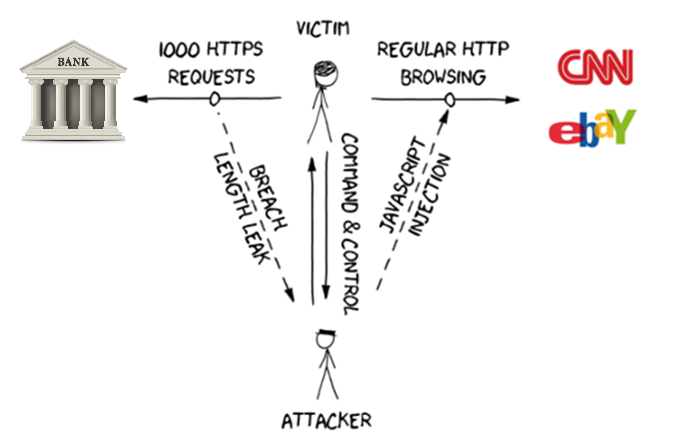
\includegraphics[width=0.48\textwidth]{figures/attack_model.png}
        \caption{The attack model}
        \label{fig:attack_model}
    \end{figure}

\subsection{A motivating example, concepts and notations}\label{subsec:terms}
We now describe a concrete example of the website in the previously described
attack to illustrate the various terms we use in the rest of this paper.  The
terms that need be explained include the \textit{rendering function} $f$,
\textit{rendered message} $m$, \textit{secret} $s$, \textit{noise} $v$,
\textit{reflection} $r$ and the distributions $\mathcal{M}$ of secrets and
$\mathcal{V}$ of noise.

In our example, the target of the attack is the website found in the URL
\textit{mail.example.com}. The victim is the user that is logged in this mail
service and whose cookies the adversary uses in his requests (and aims to learn).

The web page that the adversary exploits is
\textit{mail.example.com/search?query=attack}. This website provides a HTTP GET
parameter called \textit{query} and the adversary uses the reflection string
\textit{attack}. The HTML response is included below:

\begin{lstlisting}[basicstyle=\small\ttfamily]
<div>
    <p>You searched for: attack</p>
    <p>No results found.</p>
</div>
<div>
    Your inbox:
    <ul>
    <li>[Bank] Routing number: 123</li>
    </ul>
</div>
<div>
    <p>Current Time: 12:40:00</p>
</div>
\end{lstlisting}

The server's HTML generator is an instance of the \textit{rendering function}
$f$. This function implements the rendering of the HTML code based on
blueprints.

The output of $f$ is the \textit{rendered message} $m$. This is the generated
HTML response code that contains response data and is rendered by the user's
browser.

The HTML response contains multiple data elements. A data element can be a
\textit{secret}, \textit{noise}, \textit{static}, or a \textit{reflection}.

A \textit{secret} $s$ is any part of the response that the application wishes to
remain private. The adversary wishes to learn information about $s$. Examples of
secrets in an HTML response include private messages, email contents, financial
data, and web security elements like CSRF tokens \cite{de2011automatic}. A secret's alphabet
is generally printable text characters. In our example, the strings "Bank",
which is an email topic, and "Routing number: 123", which is the email body, are
both secrets.

A \textit{reflection} $r$ is a component crafted by the attacker and can be
adaptively transformed as the attack progresses. In our example, the HTTP GET
value "attack" of the parameter "query" is used as a reflection. This string is
included in the response in the message "You searched for: attack". This serves
as an information message for the user and reflects in every search request the
value of the GET parameter "query".

The \textit{noise} $v$ is a value that changes in every request regardless of
the requested content. Examples of noise include timestamps and ads. The noise
follows a random distribution and its alphabet consists of printable characters.
In our example, the string "12:40:00" is noise.

\textit{Static} is any content that remains unchanged across requests. Typical
examples of static data are HTML $<$div$>$ tags and CSS code. Static content is
predictable and thus irrelevant in the attack. Strings like "div", "ul", "Your
inbox:" are considered static in our example.

Secrets and reflections are chosen from the distribution $\mathcal{M}$.
$\mathcal{M}$ in our example contains all routing numbers and 4-letter strings
like "Bank".

Finally, each noise element is chosen from the distribution $\mathcal{V}$. In
our example, $\mathcal{V}$ contains all 24hr timestamps. In every request, a new
noise element is chosen from $\mathcal{V}$. In this case it is "12:40:00".

The compression function $\textrm{Com}$ is the compression algorithm used on the
HTML response plaintext. In our example, this algorithm is DEFLATE, the most
common compression algorithm in the web. The composition of $\textrm{Com}$ and
the rendering function $f$ is the encoding function $\mathcal{K}$.

The encryption function $\textrm{Enc}$ is the encryption algorithm used by the
web server during the communication. The most commonly used symmetric encryption
algorithm today is AES. We use the function $\mathcal{E}$ to describe the
composition of $\textrm{Enc}$ and $\textrm{Com}$.

The input of $\mathcal{E}$ is the message $m$ and its output is ciphertext $c$.
This ciphertext is included in the network response packets and is sniffed by
the adversary over-the-wire.

The generation of $m$, its compression and encryption and the transmission over
the network of $c$, as well as the sniffing ability of the adversary, constitute
the reflection oracle that will further described in following sections.

The adversary issues the attack in stages. In each stage he creates a pool of
reflections and makes malicious requests for each reflection in the pool. An
attack stage ends when the adversary has successfully decrypted a single
character in the secret. He then adaptively changes the reflection pool, based
on the newly stolen character, and continues similarly with the next stage.

In some cases, the adversary aims at finding a property of the secret rather
than the secret itself. This property is $g(s)$ and the guess of the adversary
is $y$. When $g(s) = y$ the adversary has successfully recognized the property
$g$ of the secret $s$. A special case of $g$ would be a predicate $Q$.

\section{Rupture: An improved attack}\label{subsec:rupture}
Our contributions include the development of a production-grade
framework for implementing this class of attacks called Rupture.
Rupture was developed as part of the work on extending the BREACH attack against
modern systems and block ciphers.

Rupture offers the ability to inject malicious code in any computer in the
network. This code issues requests to the endpoint and serves as a caller of
the reflection oracle that is the endpoint.

Furthermore, it enables the traffic inspection and analysis of packet
lengths. Encrypted network packets serve as the response $c_i$ from the
reflection oracle and the length of each packet is visible on the network and
captured.

In addition, Rupture offers multiple instances of the oracle $\mathcal{O}_R$, based
on various $Q$ described in \ref{subsec:parallel}, and enables the automated
computation of the reflection strings in each stage of the attack.

Finally, it amplifies the attack by issuing multiple requests per candidate
symbol in the alphabet $\Sigma$ in order to demonstrate better probability of
success. This is achieved by grouping requests in samplesets, where each
sampleset contains requests on a symbol in the alphabet $\Sigma$. Requests in a
sampleset may be constructed to enable optimization methods described in
\ref{subsec:blockalign} and \ref{subsec:parallel}.

The encrypted data pertaining to one response is a \textit{sample}.  The set of
samples collected for a particular work are a \textit{sampleset}. A work
represents the set of requests needed per candidate in the secret's alphabet.

The attack is conducted in \textit{rounds}. In each round, a decision is made
about the state of the attack and more becomes known about the secret. In a
round, either the next byte of the secret becomes known, or the known alphabet
is drilled down to a smaller set. In order to compare various different
candidate alphabets, the attack executes a series of \textit{batches} of data
collection for each round.

In each batch, several works are issued and samples are collected from each probability distribution
pertaining to a candidate alphabet, forming a sampleset. When samplesets of the
same amount of samples have been collected for all the candidate alphabets,
a batch is complete and the data is analyzed. The analysis compares the samples
of different candidates and decides which is optimal, i.e. which candidate is
contains the correct guess. This decision is made with some \textit{confidence},
is expressed in bytes. If the confidence is insufficient, an additional
batch of samplesets is collected, and the analysis is redone until the
confidence value surpases a given threshold.

Once enough batches have been collected for a decision to be made with good
confidence, the round of the attack is complete and more information about the
secret becomes known.

\subsection{Architecture}\label{app:rupture}
Rupture is a service-based architecture framework which contains multiple
independent components. While the components are designed to be able to run
independently on different networks or computer systems, easy instances of the
attack can be performed by running all subsystems on an individual system.

The framework assumes a \textit{target} service to be attacked. Typically
this target is a web service which uses TLS and
provides HTTPS endpoints. However, this assumption can
be relaxed and attacks against other similar protocols are possible. Any
protocol that exchanges encrypted data on the network and for which
the attack assumptions hold can in principle be attacked using Rupture. We
designed Rupture to be a good playground for experimentation for such new
attacks. Examples of other encrypted protocols for experimentation
include SMTP and XMPP.

The attack also assumes a user of the target service for which data will be
decrypted, the \textit{victim}. The victim is associated with a particular
target.

There are two underlying assumptions in our attack: The injection and the
sniffing assumptions. These are often, but not necessarily, achieved through the same means.

The injection assumption states that the adversary is able to inject code to the
victim's machine for execution. This code is able to issue adaptive requests to
the target service. Injection in Rupture is implemented by the
\textit{injector} component. The code that is injected is the \textit{client}
component.

The sniffing assumption states that the adversary is able to observe encrypted network
traffic between the victim and the target.
Sniffing is achieved through the \textit{sniffer}component.

The client must issue adaptive requests. For this purpose, it receives commands
through a \textit{command-and-control} channel. These commands are sent to the
client from the \textit{realtime} component with which the client maintains a
persistent connection.

The realtime component is only responsible for communicating with the client.
The actual decisions for the attack are driven by the \textit{backend}, which
maintains a persistent attack state. The backend stores persistent data in a
\textit{database} and receives data from the sniffer to perform analyses.

The various components are described in detail in the next sections.

\subsubsection{Client}

The client component is a Javascript code that issues requests towards a chosen
endpoint. This endpoint serves as the reflection oracle of the attack. The client
needs to be executed from the browser of the victim that the adversary is trying
to steal secrets from. That way, the victim's authentication cookies are
included in the request and the secrets are included in the
response.

The client contains minimal logic. It connects to the realtime service through
a command-and-control channel and registers itself. Then it waits
for work instructions by the command-and-control channel. The
client does not take any decisions or receive data about the progress of the
attack other than the work it is requested to do.
This allows the system to be upgraded without having to deploy a
new client at the victim's network.

As a regular user is browsing the Internet, multiple clients will be
injected in insecure pages and run under various contexts. All of
them register and maintain an open connection through a
with the realtime service. The realtime
service will activate one of them for this victim while keeping the others
dormant. The activated one will then receive work instructions. If the enabled
client dies, for example by closing the browser
tab, one of the rest of the clients will be woken up to continue the
attack.

\subsubsection{Injector}

The injector component is responsible for injecting the client to the victim's
browser. The injection is performed by ARP spoofing the local
network and forwarding all traffic in a Man-in-the-Middle manner. The fact that all HTTP
responses are infected increases robustness.

The injector component runs on the victim network and is
light-weight and stateless. It can be easily deployed on a small machine and
used for massive attacks. Multiple injectors can be deployed to different
networks, all controlled by the same central command-and-control channel.

\subsubsection{Realtime}

The realtime service is a service which awaits for work requests by clients. It
can handle multiple targets and victims. It receives command-and-control
connections from various clients which may live on different networks,
orchestrates them, and tells them which ones will remain dormant and which ones
will receive work, enabling one client per victim.

It maintains open web socket connections with clients and
connects to the backend service, facilitating the communication between the two
ends.

\subsubsection{Sniffer}

The sniffer component is responsible for collecting data from the
victim's network. As the client issues the requests, the sniffer
collects the ciphertext of the requests and responses as they
travel on the network. This encrypted data is then transmitted to the backend
for further analysis and decryption.

The sniffer exposes an HTTP API which is utilized by the backend for controlling
when sniffing starts, when it is completed, and retrieving the sniffed data.

\subsubsection{Backend}

The backend component is a Python code that controls the attack execution. It
initializes the attack and calculates the request sets that should be
collected. It is responsible for strategic decision taking, statistical
analysis of collected samples, adaptively advancing the attack, and storing
persistent data about the attacks in progress for future analysis.

It communicates with the realtime component in order to guide the client as to
what requests need to be made at each stage of the attack. Meanwhile, it orders
the sniffer to listen and report network traffic, which stored
at the end of each phase of the attack. The backend analyzes the
network data and calculates the confidence in the success for the attack. At the
end of each round, the predicate $Q$ is detected, depending on which method of
the ones described
in \ref{subsec:reflectionmethods} is used.

   \begin{figure}[thpb]
      \centering
          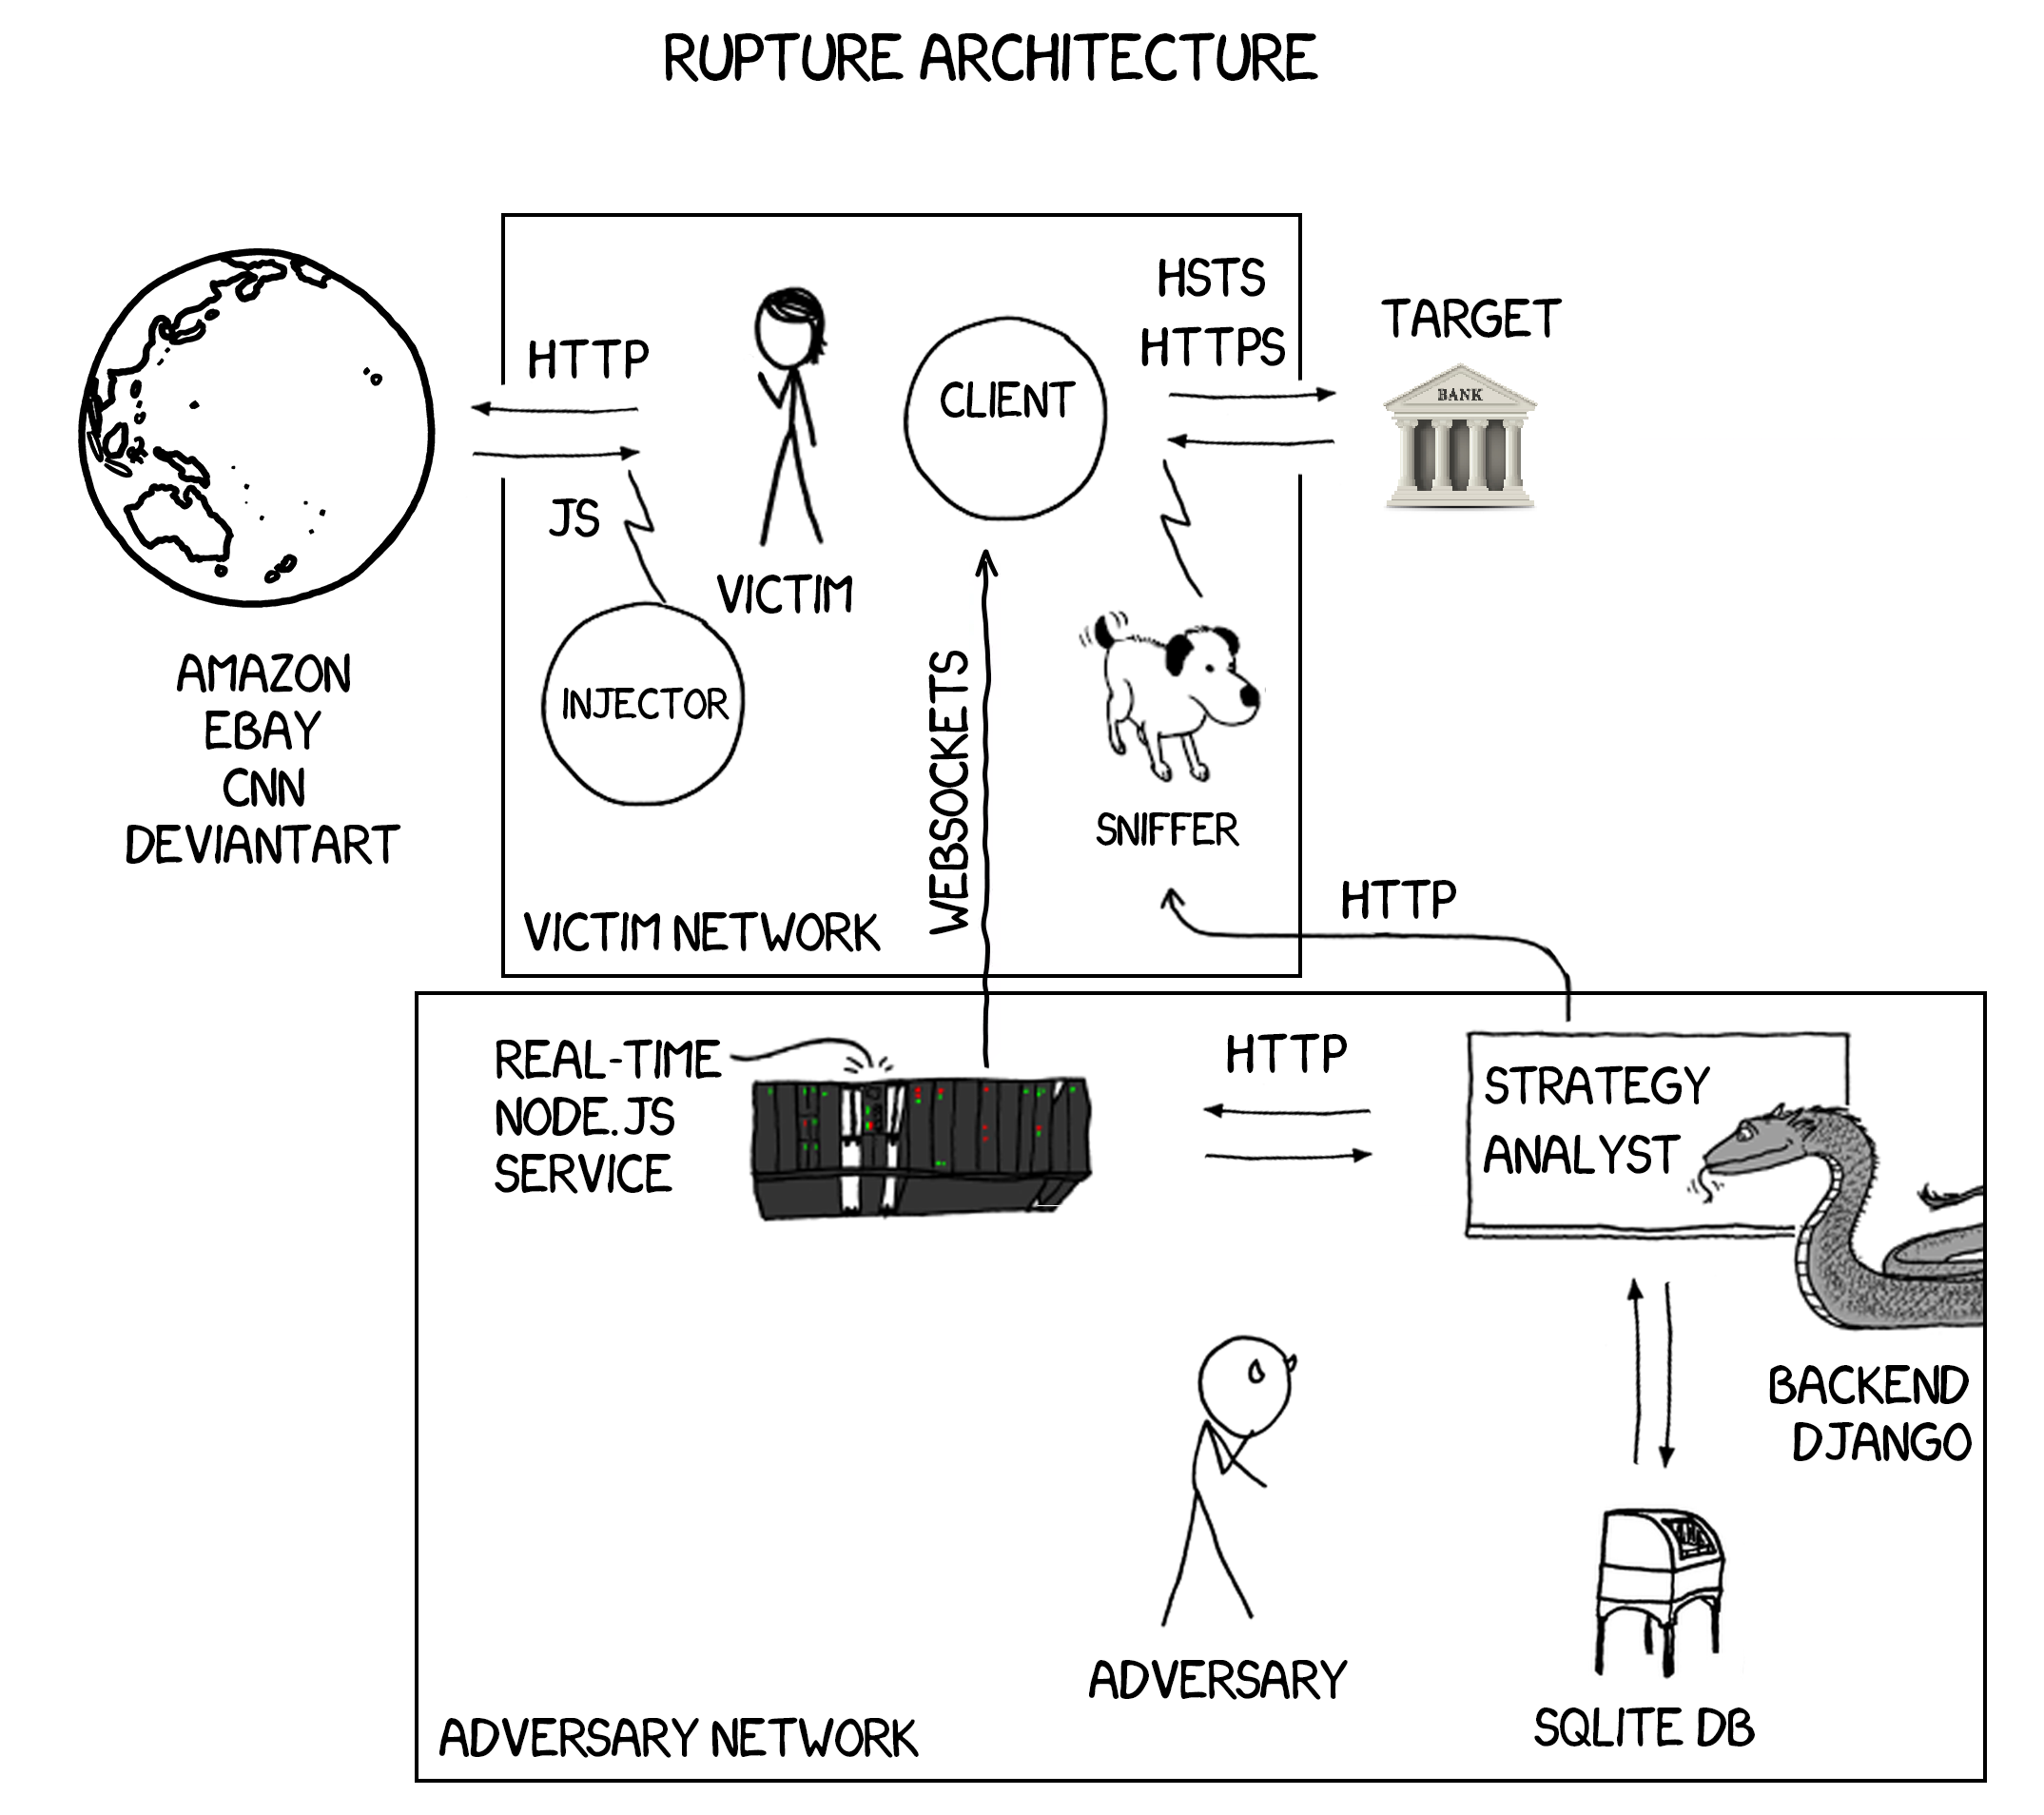
\includegraphics[width=0.48\textwidth]{figures/architecture.png}
      \caption{Rupture Architecture}
   \end{figure}

\section{Reflection security}\label{sec:refsec}

\subsection{Adaptive reflection game}\label{subsec:refsecgame}

Let $\mathcal{PE} = (Gen, \mathcal{E}, \mathcal{D})$ be a public-key
encryption scheme, $\mathcal{A}$ be an adversary and $\mathcal{S}$ be a
simulator of $\mathcal{A}$.  The game
$\text{Game}_{\text{REF-SEC}}^{\mathcal{PE},\mathcal{A}}(\lambda,  f,
\mathcal{V}, g, \mathcal{M})$ is parameterized with a rendering function $f(\cdot, \cdot,
\cdot)$, a noise distribution $\mathcal{V}$, the security parameter $\lambda$,
some function $g$ of the plaintext vector, and a distribution of secrets $\mathcal{M}_\omega$
such that for all $\omega$ and for all secrets $s$ that exist in
$\mathcal{M}_\omega$ it holds that $|s| = \lambda$. We
require that the rendering function $f$ is polynomially computable and
reversible. Notice that the distribution of secrets is parameterized with the
history of execution $\omega$.

The challenger produces a $\lambda$-bit key $(pk, sk) \leftarrow
Gen(\lambda)$. The adversary is given $pk$, $\mathcal{V}$, $g$, $f$ and
$\mathcal{M}$.
Setting $\omega = ()$, the empty vector, the challenger initially chooses
a secret $s_0 \leftarrow \mathcal{M}_\omega$.

The adversary is then allowed to run and make arbitrary calls to a reflection
oracle, which responds potentially differently to every round $i$. The oracle
is parameterized by $s_i$, the secret unknown to the
adversary.  For the reflection oracle call, the adversary chooses a reflection
string $r$ and sends it to the oracle. The oracle produces a noise string
$v \leftarrow \mathcal{V}$ and computes $m_i = f(s_i, r, v)$. Subsequently
$m_i$ is encrypted as $c_i = \mathcal{E}_\kappa(m_i)$, and $c_i$ is sent back
to the adversary. Once $m_i$ is computed, the history vector $\omega$ is updated
with the rendered message as $\omega = \omega || m_i$ where $||$ denotes the
uniquely decodable concatenation of strings, and the next secret $s_{i+1}
\leftarrow \mathcal{M}_\omega$ is chosen. Note that, because the rendering
function $f$ is reversible, the history vector $\omega$ can be used to deduce
the history of all secrets, reflections and noises.

When the adversary decides to complete the game, they output a guess $y$. The
adversary is successful if $g(\psi) = y$, where $\psi$ is the sequence
of all secrets sampled by the reflection oracle during the course of the game.

Formally, let the public key adversarial game be defined as follows:

\begin{lstlisting}[texcl,mathescape,basicstyle=\small]
def $\text{Game}_{\text{REF-SEC}}^{\mathcal{PE},\mathcal{A}}(\lambda, f, \mathcal{V}, \mathcal{M}, g)$:
    $(pk, sk) \leftarrow Gen(\lambda)$
    $\omega = ()$
    $y \leftarrow \mathcal{A}^{\text{Reflect}^{\mathcal{E}_{pk}, \mathcal{V}}}
     (\lambda, f, \mathcal{V}, \mathcal{M}, g)$
    if $y = g(\psi)$:
        return 1
    else:
        return 0
\end{lstlisting}

Where the reflection oracle provided to the adversary is as follows, where
$\psi$ is a global variable:

\begin{lstlisting}[texcl,mathescape,basicstyle=\small]
def $\text{Reflect}^{\mathcal{E}_{pk}, \mathcal{V}}(r)$:
    $s \leftarrow \mathcal{M}_\omega$
    $v \leftarrow \mathcal{V}$
    $m = f(s, r, v)$
    $\omega = \omega || m$
    $\psi = \psi || s$
    $c \leftarrow \mathcal{E}_{pk}(m)$
    return $c$
\end{lstlisting}

Let the simulator game be defined as follows:

\begin{lstlisting}[texcl,mathescape,basicstyle=\small]
def $\text{Game}_{\text{REF-SIM}}^{\mathcal{PE},\mathcal{S}}(\lambda, f, \mathcal{V}, \mathcal{M}, g)$:
    $\omega = ()$
    $y \leftarrow \mathcal{A}^{\text{ReflectSim}^{\mathcal{E}_{pk}, \mathcal{V}}}
     (\lambda, f, \mathcal{V}, \mathcal{M}, g)$
    if $y = g( \psi )$:
        return 1
    else:
        return 0
\end{lstlisting}

Where the simulator reflection oracle is configured to not answer:

\begin{lstlisting}[texcl,mathescape,basicstyle=\small]
def $\text{ReflectSim}^{\mathcal{E}_{pk}, \mathcal{V}}(r)$:
    $s \leftarrow \mathcal{M}_\omega$
    $v \leftarrow \mathcal{V}$
    $m = f(s, r, v)$
    $\omega = \omega || m$
    $\psi = \psi || s$
    return $\bot$
\end{lstlisting}

\subsection{Adversarial advantage}\label{subsec:refsecadv}

Let us now define the advantage of the adversary against a simulator:
\begin{align*}
    \text{Adv}_{\mathcal{PE}, \mathcal{A}, \mathcal{S}}&(\lambda, f, \mathcal{V}, \mathcal{M}, g) &\defeq\\
    |\Pr[\text{Game}_{\text{REF-SEC}}^{\mathcal{PE},\mathcal{A}}(\lambda, f, \mathcal{V}, \mathcal{M}, g) = 1] &-\\
    \Pr[\text{Game}_{\text{REF-SIM}}^{\mathcal{PE},\mathcal{S}}(\lambda, f, \mathcal{V}, \mathcal{M}, g) = 1]| &
\end{align*}

\subsection{Adaptive reflection security}\label{subsec:adaptiverefsec}

Given a rendering function $f(\cdot, \cdot, \cdot)$ and
a noise distribution $\mathcal{V}$, a public-key encryption scheme
$\mathcal{PE}$ is \textit{reflection-secure} if:
\begin{align*}
\forall \mathcal{M}:
\forall g:
\forall PPT \mathcal{A}:
\exists PPT \mathcal{S}:\\
\text{Adv}_{\mathcal{PE}, \mathcal{A}, \mathcal{S}}(\lambda, f, \mathcal{V}, \mathcal{M}, g) = negl(\lambda)
\end{align*}

\subsection{Non-adaptive secrets}\label{subsec:refsecnonadapt}

For the rest of this paper, we assume $s$ is chosen initially, it subsequently
remains constant and that the distribution $\mathcal{M}$ is independent of
history $\omega$. This is a special case of the above game, in the sense that we
assume that $\mathcal{M}_{()}$ is a distribution of secrets which we denote
simply $\mathcal{M}$, and subsequent random choices from $\mathcal{M}_\omega$
always return the initial secret $s$.

This simplifies the game as follows:

\begin{lstlisting}[texcl,mathescape,basicstyle=\small]
def $\text{Game}_{\text{REF-SEC}}^{\mathcal{PE},\mathcal{A}}(\lambda, f, \mathcal{V}, \mathcal{M}, g)$:
    $(pk, sk) \leftarrow Gen(\lambda)$
    $s \leftarrow \mathcal{M}$
    $y \leftarrow \mathcal{A}^{\text{Reflect}^{\mathcal{E}_{pk}, \mathcal{V}}_s(r)}(\lambda, f, \mathcal{V}, \mathcal{M}, g)$
    if $y = g(s)$:
        return 1
    else:
        return 0
\end{lstlisting}

The adversary reflection oracle is also simplified:

\begin{lstlisting}[texcl,mathescape,basicstyle=\small]
def $\text{Reflect}^{\mathcal{E}_{pk}, \mathcal{V}}_s(r)$:
    $v \leftarrow \mathcal{V}$
    $m = f(s, r, v)$
    $c \leftarrow \mathcal{E}_{pk}(m)$
    return $c$
\end{lstlisting}

And the simulator does not require an oracle for its execution:

\begin{lstlisting}[texcl,mathescape,basicstyle=\small]
def $\text{Game}_{\text{REF-SIM}}^{\mathcal{PE},\mathcal{S}}(\lambda, f, \mathcal{V}, \mathcal{M}, g)$:
    $y \leftarrow \mathcal{S}(f, \mathcal{V}, \mathcal{M}, g)$
    $s \leftarrow \mathcal{M}$
    if $y = g(s)$:
        return 1
    else:
        return 0
\end{lstlisting}

The reflection game is depicted in Figure \ref{fig:refgame}:

    \begin{figure}[thpb]
        \centering
            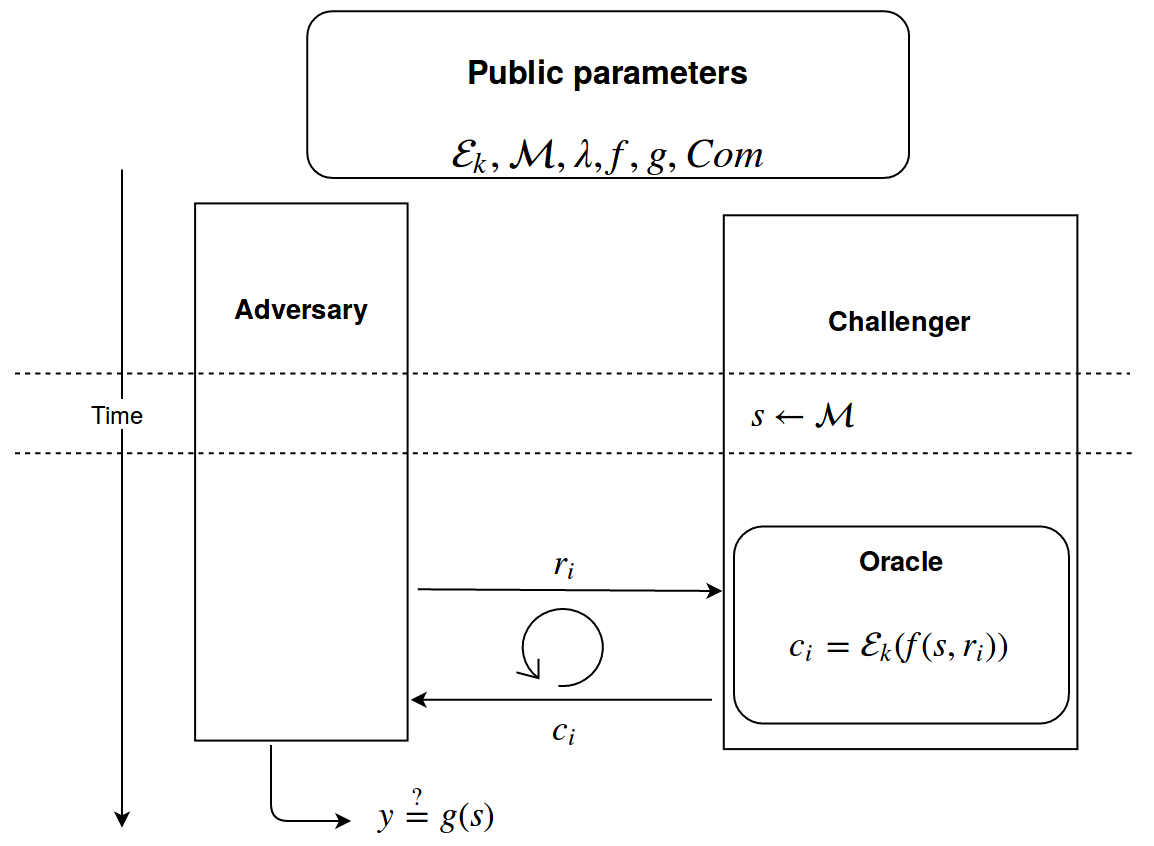
\includegraphics[width=0.48\textwidth]{figures/reflection_game.png}
        \caption{Reflection Game}
        \label{fig:refgame}
    \end{figure}

\noindent {\bf Symmetric key version.} The above game can be modified to deal
with symmetric encryption. For this, the choice of key is changed to be limited
to a secret key instead of a public and private key pair. The adversary is not
given access to any key material.  Instead, the adversary is given access to an
encryption oracle which encrypts a given message using the secret key and
returns the respective ciphertext, in addition to the existing reflection
oracle. Both oracles can be called an arbitrary number of times by the
challenger.

In the following proofs, we will assume that the game is played symmetrically.
As the attack does not pertain to the key exchange mechanism, all theorems can
be directly translated between the two versions of the game.

\begin{lemma}[Semantic security]
    Let $(Gen, K, D)$ be a length-preserving reflection-secure encryption
    scheme. Then it is also semantically secure.
\end{lemma}

\begin{proof}
    We will prove that if the scheme is not semantically secure, then it is
    necessarily not reflection secure. Assume that the scheme is not
    semantically secure. Then there will exist a PPT adversary $\mathcal{A}$
    such that for all PPT simulators $\mathcal{S}$ we have that $\mathcal{A}$
    has non-negligible advantage to $\mathcal{S}$ in the semantic security game.

    We will now construct an adversary $\mathcal{A'}$ for the reflection
    security game. $\mathcal{A'}$ operates as follows: It makes one query to
    the reflection oracle setting $r_0 = \epsilon$ and receives a response $c_0
    = K_k(s, r_0) = K_k(s) = c$. It then passes that $c$ to the semantic
    security adversary $\mathcal{A}$. It answers all encryption and decryption
    queries of the semantic security adversary by relaying them to its own
    encryption and decryption oracle. Finally, when the semantic security
    adversary outputs $y = y'$, this $y'$ is output by the reflection security
    adversary. Note that $\mathcal{A}$ cannot distinguish whether they are
    playing against the actual semantic security game or being simulated by the
    reflection security adversary, as their view is identical. Therefore:

    \begin{equation}
        Pr[Game_{REF-SEC}^{\mathcal{A'}} = 1] = Pr[Game_{SEM-SEC}^{\mathcal{A}} = 1]
    \end{equation}

    It remains to prove that $\mathcal{A'}$ has significant advantage against
    any reflection simulator $\mathcal{S'}$. Indeed let $\mathcal{S'}$ be any
    reflection game simulator. We will construct a simulator $\mathcal{S}$ for
    the semantic security game. Initially, the simulator $\mathcal{S}$ receives
    the length of the ciphertext $|c|$. They then simulate the reflection game
    simulator $\mathcal{S'}$ as follows. Upon receiving query $r_i$ from the
    reflection game simulator, they answer with $|c| + |r_i|$. When the
    reflection security adversary outputs $y' = y$, this $y$ is output by the
    semantic security simulator. We observe that the reflection game simulator
    $\mathcal{S'}$ cannot distinguish whether they are playing against the
    actual simulated reflection game or being simulated by the semantic
    security simulator. To see this, note that from the length preservation
    assumption we have that $|c| + |r_i| = |K(s, r_i)| = |K(s', r_i)| =
    |K(0^{|s|}, r_i)|$. Therefore:

    \begin{equation}
        Pr[Game_{SEM-SIM}^{\mathcal{S}} = 1] = Pr[Game_{REF-SIM}^{\mathcal{S'}} = 1]
    \end{equation}

    From the assumption that the scheme is not semantically insecure, we know
    that:

    \begin{align*}
        |Pr[Game_{SEM-SEC}^{\mathcal{A}} = 1] - Pr[Game_{SEM-SIM}^{\mathcal{S}} = 1]| =\\
        Adv_{\mathcal{A}, \mathcal{S}} = \text{non-negl}
    \end{align*}

    And therefore, replacing both probabilities with their equals:

    \begin{align*}
        |Pr[Game_{REF-SEC}^{\mathcal{A'}} = 1] -
        Pr[Game_{REF-SIM}^{\mathcal{S'}} = 1]| =\\
        Adv_{\mathcal{A'}, \mathcal{S'}} = \text{non-negl}
    \end{align*}
\end{proof}

\section{The security of compression}\label{sec:comsec}

\subsection{The interdependence assumption}\label{subsec:interdependence}

Let $\bar{\mathcal{M}}$ be a joint distribution from which the random variables
$(s, r)$ are drawn. We say that $s$ and $r$ are interdependent when there exist
$s_1, r_1$ and $s_2, r_2$ in the support of $\bar{\mathcal{M}}$ with $s_1 \neq
s_2$ such that:

\begin{align*}
    \Pr[(s, r) = (s_1, r_1)] &< \Pr[(s, r) = (s_1, r_2)]
\land\\
    \Pr[(s, r) = (s_2, r_1)] &> \Pr[(s, r) = (s_2, r_2)]
\end{align*}

Where the pair $(s, r)$ is drawn from the joint distribution
$\bar{\mathcal{M}}$.

It is clear that when two random variables $s$ and $r$ exhibit interdependence,
they must necessarily be dependent random variables. To see that
interdependence is a stronger version of dependence, observe that in the case
of dependence, the probability for some $s = s_1$ conditioned on $r = r_1$ is
necessarily different from the probability for some $s = s_2$ conditioned on $r
= r_2$. In interdependence, it can be seen that we additionally require the
event $s = s_1$ which was less probable than the event $s = s_2$ under the
condition $r = r_1$ to become more probable than $s = s_2$ under the condition
$r = r_2$.

We observe that commonly compressed texts such as HTML content exhibit
interdependence almost everywhere. To be more precise, if we sample, for
example, digrams (two-letter sequences) in HTML content of popular websites and
treat this two-letter sequence $\phi = (s, r)$ of the two characters $s$ and
$r$ as a random variable $\phi$, we notice that $s$ and $r$ are dependent
variables and in fact interdependent. Similarly when sampling two-word sequences
$\phi = (s, r)$ of the two words $s$ and $r$ from English literature, then $s$
and $r$ are interdependent. The same occurs for digrams in English. This
straightforward fact is supported by extensive statistical analyses in the
scientific literature such as \cite{mayzner1965tables}.

While the interdependence assumption is a general notion observed in all common
plaintexts, it is suitable to mention here how these ideas will emerge as we
mount our attack. In a plaintext $(s, r)$ in which the attacker controls some
reflection string $r$ and wishes to obtain information about some secret string
$s$, she wishes to distinguish between the cases $s = s_1$ and $s = s_2$ of two
different secrets $s_1$ and $s_2$, i.e. between the instances $(s_1, r)$ and
$(s_2, r)$. By measuring the difference in the probability of $(s, r)$
occurring for $r = r_1$ and $r = r_2$, the attacker can distinguish which value
of $s$ is in use. If $s = s_1$, then the attacker will observe the inequality
$\Pr[(s, r) = (s_1, r_1)] < \Pr[(s, r) = (s_1, r_2)]$, but when $s = s_2$, the
attacker will observe the different inequality $\Pr[(s, r) = (s_2, r_1)] >
\Pr[(s, r) = (s_2, r_2)]$.

The necessity of the assumption that the plaintext being compressed follows an
interdependent distribution will become clear shortly, when we introduce our
definition of compression functions. This will also immediately hint at how the
attacker is able to perform these measurements of probability inequalities
indirectly by observing ciphertext lengths.

\subsection{Composing with compression}\label{subsec:comcompose}

We now shift our interest to algorithms which compose compression and
encryption. We define the composition of a compression algorithm with a
rendering function and an encryption algorithm.

The encryption scheme above is treated as a composition of a
compression and encryption algorithm:
\begin{equation*}
    \mathcal{E} = \textrm{Enc} \circ \textrm{Com}
\end{equation*}

$\textrm{Com}$ is any polynomially computable reversible function that takes an
input string and outputs a new string: $\textrm{Com}: \{0, 1\}^* \leftarrow \{0,
1\}^*$.

$\textrm{Enc}$ denotes an encryption function. We stress our important
assumption that $\textrm{Enc}$ is defined on $\{0, 1\}^*$ and not on some
fixed-length input.

The composition of the compression function $\textrm{Com}$ and the rendering function $f$
is defined:
\begin{equation*}
    \mathcal{K} = \textrm{Com} \circ f
\end{equation*}

We call $\mathcal{K}$ an editing function. For the rest of the paper, we treat
$\mathcal{K}$ as a compression function.

\subsection{Compression idealness}\label{subsec:com_idealness}

We now move on to define the notion of compression idealness.

Let $\mathcal{K}$ be a function defined on some domain and with output space
all strings $\{0, 1\}^*$, and let $\bar{\mathcal{M}}$ be a distribution whose
support is a subset of the domain of $\mathcal{K}$.  We say that $\mathcal{K}$
is an ideal compression function with respect to the distribution
$\bar{\mathcal{M}}$ when for every $w_1, w_2$ in the support of
$\bar{\mathcal{M}}$ we have:

\begin{equation*}
\Pr[w = w_1] < \Pr[w = w_2] \iff \lvert\mathcal{K}(w_1)\rvert > \lvert\mathcal{K}(w_2)\rvert
\end{equation*}

Where $w$ is a random variable drawn from $\bar{\mathcal{M}}$.

The intuitive notion behind compression idealness is that the encoding
function is somehow perfectly aware of the input distribution. It
exploits this knowledge of the input space to encode each possible
input in an ideal way – more often occurring plaintexts are compressed
better, i.e. in shorter length, than rarely occurring plaintexts.
Practical compression functions are not perfectly ideal, because the
distribution of plaintexts they try to cover is broad and ill-defined.
However, such compression functions try to learn the distribution of
the plaintext they are about to compress by observing frequencies of
occurrences and taking advantage of them.

We now turn our attention to two specific compression functions, the
LZ77 and Huffman function. These two compression functions are of
interest for two reasons. First, they are representative of the way
typical lossless compression functions work internally, by taking
advantage of letter frequencies (Huffman) or letter-sequence
repetitions (LZ77). Second, they are the ones almost exclusively used in
practice. The DEFLATE algorithm \cite{deutsch1996deflate}, which is a composition of LZ77 and
Huffman, is the algorithm used in gzip, which is prevalent on the
modern web. In 2016, 98.85\% of websites that enabled compression used
some form of gzip. We argue that both LZ77 and Huffman are nearly
ideal compression functions. The complexity of the Huffman and
especially the LZ77 algorithms arises from many intricate technical
details, such as, for instance, the sliding window size of LZ77. These
details make it impractical to deal with these functions in analytical
proofs.

We support our idealness claims in an experimental manner. Our experiment
measured the compression performance of the Huffman and an ideal function on a
text of English literature\footnote{The screenplay of the movie "The Social
Network".}. First, we calculated the occurences of each character (letters and
digits) in the text. Second, we generated the Huffman
table for this text and the table of an ideal function based on the character
frequencies. Each character is represented by a bitstream in both tables. Figure
\ref{fig:huffman_idealness} depicts the length of the bitstreams of characters
in descending order of occurencies for both the ideal and the Huffman functions.

    \begin{figure}[thpb]
        \centering
            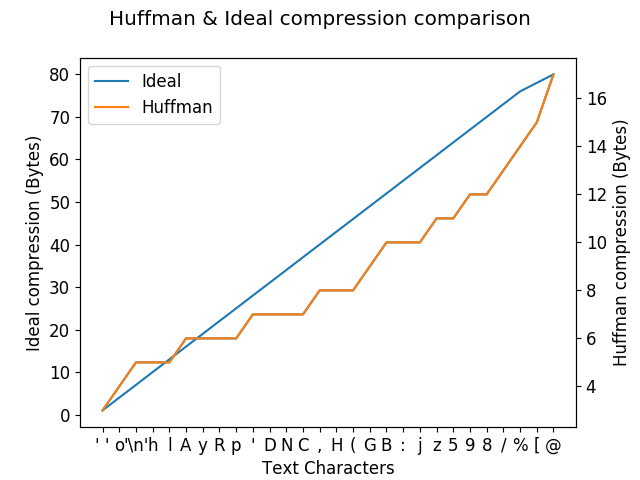
\includegraphics[width=0.48\textwidth]{idealness_experiments/huffman_idealness.png}
        \caption{Comparison between Huffman and ideal compression}
        \label{fig:huffman_idealness}
    \end{figure}

\subsection{Length monotonicity}\label{subsec:lenmonotone}

An important assumption for our attack is that the encryption function
$\textrm{Enc}$ is \textit{length monotonic}. Specifically, for any keys $k_1
k_2$ in the key generating function space and string messages $m_1, m_2$:

\begin{equation*}
\begin{split}
|m_2| > |m_1|
\Rightarrow
|\textrm{Enc}_{k_1}(m_2)| \geq |\textrm{Enc}_{k_2}(m_1)|
\end{split}
\end{equation*}

If the last inequality becomes strict, we call the encryption function
\textit{strictly length monotonic}.

A practical instance of a length monotonic encryption function is AES \cite{standard2001announcing}.
Stream ciphers can be treated as strictly monotonic to the bit level.

\section{Compressibility with respect to predicates}\label{sec:propertycom}
In this section we will define compressibility with respect to predicates. We
show that all ideal compression functions that exhibit interdependence are
compression detectable by a reflection vector $\overbar{r}$ with respect to a
predicate $Q$ and a distribution $\mathcal{M}$

Let $\mathcal{M}$ be a plaintext distribution and $Q(s)$ be a predicate on the
plaintext $s$ drawn from $\mathcal{M}$. Furthermore, we require that $Q$ is not a
trivial predicate; that is, there must exist elements for which $Q$ is true and
others for which it is false.  Let us use $\mathcal{M}_Q$ to denote the
distribution $\mathcal{M}$ conditioned on the predicate $Q$.

For the specific property $Q$ and plaintext distribution $\mathcal{M}$, define:
\begin{equation*}
    \pi \defeq max(\Pr[Q(s)], 1 - \Pr[Q(s)])
\end{equation*}

Where $s$ is drawn from $\mathcal{M}$.

Let $\mathcal{V}$ be a noise distribution from which a pair of noises
$\overbar{v} = (v_1, v_2) \leftarrow \mathcal{V}^2$ is drawn.  Let $\overbar{r}
= (r_1, r_2) \in \mathcal{M}^2$ be a reflection string pair, $\mathcal{K}$ be an ideal
compression function, $f$ be a rendering function, and let $\alpha(\lambda)$ be
a non-negligible function.

We now examine how the lengths of compressing a secret $s$ rendered with
reflection strings $r_1$ and $r_2$ respectively compare.

The predicate $Q$ partitions the set $\mathcal{M}$ into two partitions
$\mathcal{M}_Q$ and $\mathcal{M}_{\lnot Q}$. We are interested in reflection
string pairs $\overbar{r} = (r_1, r_2)$ for which the comparison direction
depends on which partition $s$ belongs to.  The direction of comparison can
also depend on a noise vector $\overbar{v}$.  If $s \in \mathcal{M}_Q$, it
should compress better when reflection $r_1$ is used as compared to when $r_2$
is used. On the contrary, if $s \in \mathcal{M}_{\lnot Q}$, the opposite
direction should occur.  If this is the case for the selected reflection pair
and noise pair, we say that $Q$ compares favourably under $\overbar{r},
\overbar{v}$:

\begin{equation*}
\begin{split}
    cpr^Q_{\kappa}(s, \overbar{r}, \overbar{v})
    \defeq\\
    \begin{cases}
        |\mathcal{K}(s, r_1, v_1)| < |\mathcal{K}(s, r_2, v_2)| &\text{ if } Q(s)\\
        |\mathcal{K}(s, r_1, v_1)| \geq |\mathcal{K}(s, r_2, v_2)| &\text{ otherwise}
    \end{cases}
\end{split}
\end{equation*}

The reflection pair $\overbar{r}$ \textit{detects} predicate $Q$ under
compression function $\kappa$ over the secret distribution $\mathcal{M}$ and
the noise distribution $\mathcal{V}$ with advantage $\alpha$ when the
comparison is favourable for both $s_1$ drawn from $\mathcal{M}_Q$ and $s_2$
drawn from $\mathcal{M}_{\lnot Q}$. Formally, we define the predicate
$dtc_\alpha(Q, \overbar{r}, f, \textrm{Com}, \mathcal{M}, \mathcal{V})$ as follows:

\begin{align*}
    \Pr
        [cpr^Q_{\kappa}(s_1, \overbar{r}, \overbar{v}) \land
         cpr^Q_{\kappa}(s_2, \overbar{r}, \overbar{v})]
    \geq\\
    \pi + \alpha(\lambda)
\end{align*}

Where $s_1$ is drawn from $\mathcal{M}_Q$, $s_2$ is drawn from
$\mathcal{M}_{\lnot Q}$, and $v_1, v_2$ are drawn from $\mathcal{V}$.

We call $Q$ \textit{compression-detectable} with an advantage $\alpha$ if a
pair $\overbar{r} = (r_1, r_2)$ exists, such that $dtc_\alpha(Q, \overbar{r},
\kappa, \mathcal{M}, \mathcal{V})$ holds. Furthermore we require that such a
pair $\overbar{r}$ is polynomially computable. That is, there exists some
polynomial-time functionality $\mathcal{O}_R(\kappa, Q, \mathcal{M},
\mathcal{V})$ which produces an $\overbar{r}$ such that $dtc_\alpha(Q,
\overbar{r}, \kappa, \mathcal{M}, \mathcal{V})$ holds.

The compression-detectability property exists in all common compression
functions as long as $s$ and $r$ compress in the same context. We will now
prove the fact that all compression functions which are ideal under some
distribution $\bar{\mathcal{M}}$ exhibit compression-detectability of some
predicate $Q$.

\subsection{Good compression allows predicate detection}

We now move on to show that all good compression functions exhibit
compression-detectability of some predicate. In intuitive terms, this means
that if a compression function compresses well enough, it will necessarilly
allow one part of the plaintext to affect how another part of the plaintext
compresses. An attacker that is able to measure how well a string compresses
can use this to detect a predicate on the second part of the plaintext by
changing the first part of the plaintext.

More specifically, we model our plaintext input to the compression function as
the usual pair $(s, r)$ consisting of the secret string $s$ and reflection
string $r$. When $(s, r)$ are encoded by a compression function $\kappa$ ideal
under some plaintext distribution $\bar{\mathcal{M}}$, a simple predicate
allows the distinction between two secrets $s_1$ and $s_2$ using a reflection
pair $(r_1, r_2)$.

In the following theorem, we prove compression detectability of a predicate
with the following simplifications. First, we make the assumption that the
resulting reflection pair $(r_1, r_2)$ is computable; second, for this proof
we ignore the existence of noise.

\begin{lemma}[Good compression is detectable]
Let $\kappa$ be an ideal compression function with respect to some
interdependent distribution $\bar{\mathcal{M}}$. Then there exists
some compression-detectable predicate $Q$ for $\kappa$.
\end{lemma}

\begin{IEEEproof}

From the fact that $\bar{\mathcal{M}}$ is interdependent, we have that:

\begin{align*}
    \Pr[r = r_1|s = s_1] < \Pr[r = r_2|s = s_1]&\land\\
    \Pr[r = r_1|s = s_2] > \Pr[r = r_2|s = s_2]&
\end{align*}

Using the fact that $\kappa$ is ideal with respect to this distribution,
we deduce that:

\begin{align*}
    |\kappa(s_1, r_1)| > |\kappa(s_1, r_2)|&\land\\
    |\kappa(s_2, r_1)| < |\kappa(s_2, r_2)|&
\end{align*}

We then define $Q(s)$ to be the predicate "$s = s_1$". This partitions
$\mathcal{M}$ into the distributions $\mathcal{M}_Q$ and
$\mathcal{M}_{\lnot Q}$ both of which are non-empty, as $\mathcal{M}_Q$
contains $s_1$ and $\mathcal{M}_{\lnot Q}$ contains $s_2$. From the fact that
$Q$ is not trivial, we deduce that $\pi < 1$.

Observe, then, that letting $\bar{r} = (r_1, r_2)$ we obtain:

\begin{align*}
    \Pr[cpr^Q_{\kappa}(s_1, \bar{r}, \kappa, \mathcal{M})
    \land
    cpr^Q_{\kappa}(s_2, \bar{r}, \kappa, \mathcal{M})] = 1
\end{align*}

This completes the proof.

\end{IEEEproof}

\subsection{One-shot attack}

\begin{lemma}[Compression attack]

Let $\textrm{Com}$ be a compression function, $\textrm{Enc}$ be a strictly length-monotonic
encryption function, $f$ be a rendering function and $Q$ be a plaintext
predicate detectable with non-negligible advantage $\alpha$ over plaintext
distribution $\mathcal{M}$.

Then:
\begin{align*}
    \exists \alpha \text{ non-negl}:
    \forall \textrm{Enc}:
    \exists g:\\
    \exists PPT \mathcal{A}:
    \forall PPT \mathcal{S}:\\
    \text{Adv}_{\mathcal{SE}(\textrm{Enc}, \textrm{Com}), \mathcal{A}, \mathcal{S}}
    (\lambda, f, \mathcal{M}, g) = \alpha(\lambda)
\end{align*}

\end{lemma}

For a full proof, see Appendix A.

\subsection{Amplified attack}\label{subsec:amplification}

We can now amplify the attack to achieve a better probability of success by a small modification in our adversary.
The amplification is parameterized by an odd parameter $k$.

Let the amplification adversary be defined as follows:

\begin{lstlisting}[texcl,mathescape,basicstyle=\small]
def $\mathcal{A}(Q, \mathcal{M})$:
    $(r_1, r_2) \leftarrow \mathcal{O}_R(\textrm{Com}, f, Q, \mathcal{M})$

    $low = 0$
    $high = 0$

    for $i$ = $0$ to $k$:
        $l_1 = |\text{Reflect}^{\mathcal{E}_{pk}}_s(r_1)|$
        $l_2 = |\text{Reflect}^{\mathcal{E}_{pk}}_s(r_2)|$

        if $l_1 < l_2$:
            $low = low + 1$
        else:
            $high = high + 1$

    if $low > high$:
        return True
    else:
        return False
\end{lstlisting}

\begin{lemma}[Amplification]

Under the assumptions of the Compression Attack Theorem against $f, \textrm{Com}$
and compression-detectable predicate $Q$ with non-negligible
detectability margin $\alpha(\lambda)$,
the amplified adversary achieves an arbitrarily large advantage
against a non-negligible subset of elements, the
\textit{amplifiable elements} distinguished by predicate $Amp$.
\begin{align*}
    \forall \textrm{Enc}:
    \exists g:\\
    \exists PPT \mathcal{A}:
    \forall PPT \mathcal{S}:\\
    \exists Amp:
    \exists B \text{ non-negl}:
    \exists C \text{ negl}:\\
    \Pr_{s \leftarrow \mathcal{M}}[Amp(s)] = B(\lambda) \land\\
    \text{Adv}_{\mathcal{SE}(\textrm{Enc}, \textrm{Com}), \mathcal{A}, \mathcal{S}_{Amp}}
    (\lambda, f, \mathcal{M}, g) = 1 - \pi - C(k)
\end{align*}

\end{lemma}

The complete proof can be found in Appendix A.

\section{Rupture Optimizations}\label{subsec:optimizations}

\subsection{Block alignment}\label{subsec:blockalign}
Block ciphers are \textit{length monotonic}, but not \textit{strictly length
monotonic}, as described in section \ref{subsec:lenmonotone}. Specifically, the
length of the encrypted text is rounded up to a product of $\mu$-bits, where
$\mu$ is the block size. This results in plaintext length difference between two
messages not always resulting in length difference between the respective
encrypted ciphertext.

We bypass this problem by using block alignment techniques
\cite{moller2014poodle}. This method demands issuing multiple requests to the
reflection oracle while including artificial noise.  In each request $r_{i, c}$
for each candidate $c$ in the secret alphabet, we add increasing artificial
noise. That way, all $r_{1, c}$ for the candidates will contain one
character of alignment noise, $r_{2, c}$ two characters and so forth.
Therefore, for some alignment noise length $a \in [0, \mu)$ the reflection
of the correct candidate will be $(\delta*\mu)$ and for all incorrect
candidates $(\delta*\mu)+1$. In that case, the incorrect candidates result
in one more block compared to the correct one. This ensures that one out of
$\ceil{\mu / |r_i|}$ requests will result in a block distinction between the
alphabet candidates. Figure \ref{fig:block_alignment} depicts the block
alignment technique intuitively.

   \begin{figure}[thpb]
      \centering
          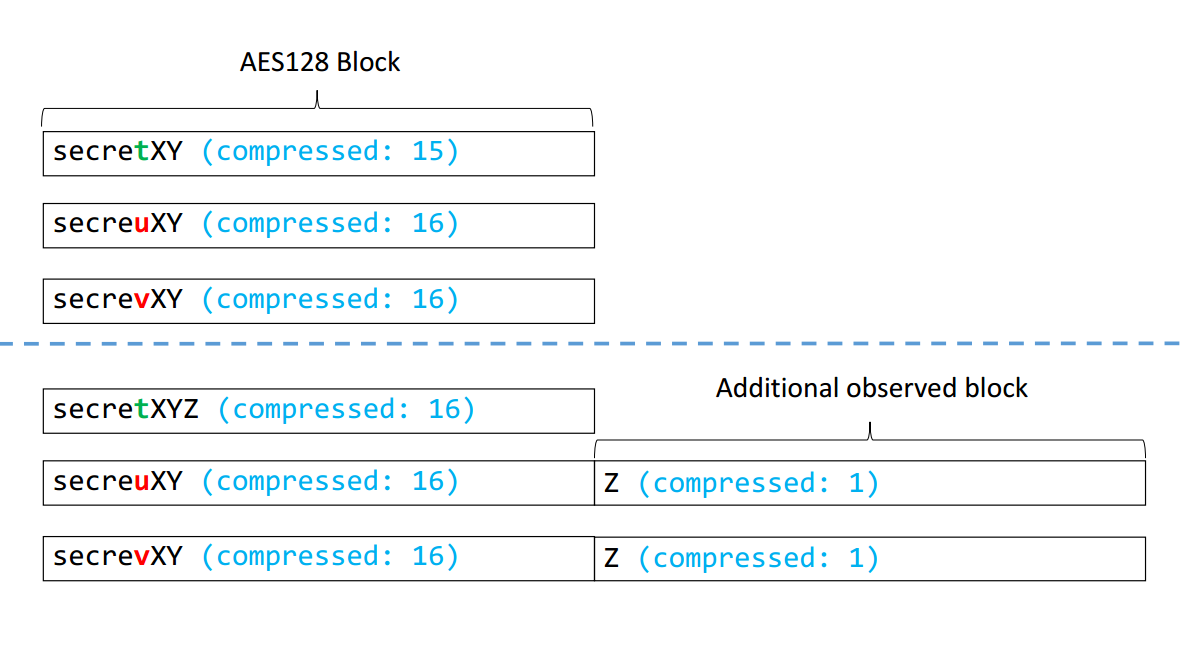
\includegraphics[width=0.48\textwidth]{figures/block_alignment.png}
      \caption{The block alignment method}
      \label{fig:block_alignment}
   \end{figure}

\subsection{Reflection computation methods}\label{subsec:reflectionmethods}
The reflection strings $r$ should be polynomially computable, as defined in
\ref{subsec:propertycom}. BREACH is parameterized with an alphabet of ASCII
symbols $\Sigma$ for each character of the secret and a successful attack should
distinguish a single character of the alphabet through a series of requests.

The first method of issuing these requests is serial. Each request contains to a
single character of the alphabet and an attack phase is completed when requests
have been issued for the entire alphabet. The complexity of this attack is
$\mathcal{O}(|\Sigma|)$ and the round ends by finding a character of the secret.
This method is similar to how BREACH previously worked.

The second method of attack is divide and conquer. In each phase the alphabet is
divided into two subsets $\Sigma_1$ and $\Sigma_2 = \Sigma \setminus \Sigma_1$,
where $|\Sigma_1| = |\Sigma_2| = \ceil{|\Sigma| / 2}$. The reflection string for
$\Sigma_1$ consists of $|\Sigma_1|$ substrings separated by an annotation symbol
$\beta$.  Each substring consists of the known prefix concatenated with a
candidate in $\Sigma_1$.  For example, if $\Sigma_1$ is $\{"1", "2"\}$ and the
known prefix is "abc", using "-" as $\beta$ the reflection is: "abc1-abc2". The
reflection string for $\Sigma_2$ is constructed similarly.

As long as the prefix of the secret is \textit{compression-detectable} by each
substring of the reflection, the end of each phase marks the choice of subset
$\Sigma_i$ that contains the correct alphabet symbol.  When $|\Sigma| = 1$ the
round is complete. Each round reduces the alphabet by half, so the complexity of
this attack is $\mathcal{O}(log|\Sigma|)$. Figure \ref{fig:divide_and_conquer}
depicts the reflection sequence for the case when the alphabet consists of
number digits.

   \begin{figure}[thpb]
      \centering
          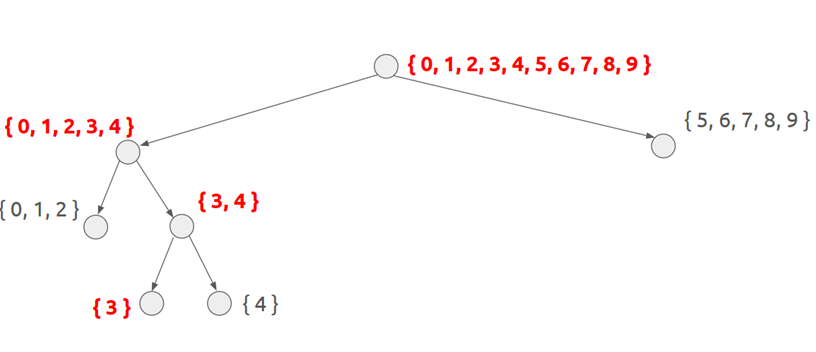
\includegraphics[width=0.48\textwidth]{figures/divide_and_conquer.png}
      \caption{The divide \& conquer method}
      \label{fig:divide_and_conquer}
   \end{figure}

\subsection{Request parallelization}\label{subsec:parallel}
The reflection oracle is generally synchronous, although it may be able to
handle multiple parallel requests from the adversary.  This is the case in
BREACH.  Modern web servers are able to handle multiple parallel requests and
browsers can issue a certain amount of parallel requests per domain. This
functionality enables the adversary to issue multiple parallel requests per
symbol in alphabet $\Sigma$ and efficiently reduce the execution time of the
attack.

\subsection{Request soup}
Previous sections demonstrated the need for multiple requests per reflection
string $r_i$. However, communication with the reflection oracle is time
expensive, so it may be preferable to issue multiple requests for a candidate
and treat them as a set rather than separately.

This technique is useful in the case of BREACH. A request set consists of
requests for a symbol $s_i$ in alphabet $\Sigma$. Bigger request sets result in
less time delay and the adversary can measure the mean length over the number of
requests in the set.

\section{The defense}\label{sec:defense}
Keeping in mind our theoretical model, we determine the key elements that make these
attacks possible.

We propose a defense, \textit{context hiding}, that mitigates a class of
practical compression side-channel attacks such as CRIME, TIME, BREACH, Rupture,
and HEIST. The full plaintext recovery these attacks perform is no longer
possible when our defense is applied.

\subsection{Hardness of defending}
First of all, observe that there is a trivial method of defense, and that is
disabling compression completely.

However, defending against an adversary by modifying $f$ is hard in general. We
note that $f$ is required to be polynomially reversible, meaning it must contain
enough information to recover $s$. Because $Com$ must be able to decrease the
length of various plaintexts, it can output plaintexts of different lengths
dependent on $s$. Therefore, if $Com$ is adversarial, it can easily leak
information through the encryption function $Enc$ by using its output length. As
such, any attempt to generally defend against all compression functions $Com$ is
necessarily futile.

However, the fact that it is theoretically difficult to define a generic defense
should not discourage us from pursuing a practical defense that applies in
practice given the specific compression functions currently in use in the
real-world.  In this direction, we give a series of arguments for why we believe
our defense method is secure based on our previously developed theory.

\subsection{Attack elements from a defense perspective}
The basic problem that needs be solved is the compression detectability of the
predicate $Q$ under this class of attacks. In order to eliminate detectability,
it should be made impossible for any pair of reflections $\overbar{r}$ to detect
$Q$ under the compression function $\textrm{Com}$ and the rendering function
$f$. In order to achieve this there exist two options - either change the
compression or the rendering function.

The next step is determining what what kind of changes are needed. We therefore
consider the notions that make detectability possible. These notions are
compression idealness and interdependence. The first is part of the composition
of $\textrm{Com}$ and $f$ whereas the second is part of $f$. That said, removing
either of these notions from the functions will strip the adversary the ability
to detect $Q$.

The first choice is forcing the compression function to act non-ideally in the
cases of secrets. Proposed defenses like disabling compression for annotated
secrets incorporate this exact idea.

The second choice is removing the interdependece between reflections and
secrets. In order to achieve that we need to decorrelate the probability of
secrets and reflections. A method that acts similarly is secret masking,
described in section \ref{subsec:masking}. Context hiding also builds on this
option and is described in the following sections.

\subsection{Context hiding properties}

Context hiding is built on the premise of separating secrets in a per-origin
manner in order to avoid cross-compression. In order to achieve this we define
what constitutes an origin and what properties same-origin secrets share.

\subsubsection{Origins}
An origin is a uniquely identifiable party that generates content. A party can
be either a physical entity, like a user, or an application. It is important to
properly identify the party that generated a piece of content, as the definition
of origins reflects the amount of knowledge on same-origin content.

\subsubsection{Same-origin secrets}
After defining the origins, we separate the secrets as content pieces assigned
to origins. All secrets assigned to an origin should have been generated by the
party that this origin identifies. An immediate result of this definition is
that anyone with access to a secret $s$ of origin $o$ also has access to all
other secrets $s'$ of the same origin $o$.

\subsection{Context hiding functionality}
Our defense method disables cross-compression by applying a simple substitution
cipher derived from a random permutation of the plaintext alphabet.

Firstly, we identify the origins of the plaintext $m$ and store them in the
array $origins$. Each secret $s_i$ in $m$ is identified by its origin. Each
origin is uniquely identified by an integer in range $[0, |origins|-1)$.

Secondly, we identify the alphabet for each origin. An origin's alphabet is the
set of characters of all secrets in this origin. For each origin, we generate a
random permutation of the origin's alphabet and store it in the array
$permutations$. The first element in the $permutations$ array corresponds to the
first origin in the $origins$ array and so forth.

In order to secure the secret $s$ we apply a hiding function. This function
\textit{hide} takes two arguments, the secret $s$ and the permutation $p$ of the
secret's origin. It applies the substitution cipher on each character in $s$ and
returns the permuted secret $s'$. The substitution cipher is implemented in the
function $Permute_p(c)$, which returns the $i$-th character in $p$, $i$ being
the index of $c$ in the clear alphabet.

\begin{lstlisting}[texcl,mathescape,basicstyle=\small]
def hide($s, p$):
    $s' = ''$
    for $ch \in s$:
        $s' = s' || Permute_p(ch)$
    return $s'$
\end{lstlisting}

The protected secret $s'$ is annotated by the special characters
$\beta_{start}^i$, $\beta_{end}^i$ that mark the start and the end of any
substring that needs to be unpermuted and are unique per origin. The output $m'$
that is produced after hiding all secrets consists of all permuted texts
concatenated with the permutation array $permutations$.

The initial secret $s$ can be retrieved from the protected secret $s'$ using the
\textit{unhide} function. This function takes $s'$ and permutation $p$ of the
secret's origin, applies the reverse permutation on $s'$, and returns the
unpermuted secret $s$.

\begin{lstlisting}[texcl,mathescape,basicstyle=\small]
def unhide($s', p$):
    $s = ''$
    for $ch \in s'$:
        $s = s || Permute_p^{-1}(ch)$
    return $s$
\end{lstlisting}

In our theoretical model, we assume that there exists a single secret. However,
in this section we generalize this and, in practice, the reflection $r$ and the
secret $s$ are handled as two secrets that have different origins. The fact
that $s$ and $r$ are permuted every time an oracle call is made makes it
impossible for an adversary controlling $r$ to learn information about $s$.

Our defense is implemented in the application layer and is opt-in. We choose to
update the rendering function $f$ instead of the compression function
$\textrm{Com}$ as it is easier for web developers to incorporate it in their
applications. Our proposal requires no changes in the underlying compression
algorithms in the web server such as Apache's mod\_deflate, which would require
a huge engineering effort. Instead, it only requires modifications in the web
application layer and can be relatively easily incorporated in existing
applications.

\section{CTX: Mitigating BREACH with Context Hiding }\label{sec:ctx}

\subsection{Implementation}
Our contributions include the development of the CTX defense. CTX is an
implementation of the context hiding method described in the previous section
for HTML web pages.

It is up to the application developer to decide which portions of the response
are sensitive and must be protected as secrets. Sensitive data does not only
include high-value secrets such as passwords and CSRF tokens, but also any data
that the developer wishes to keep private. Some examples are the bodies of email
messages, chat messages, or the contents of documents and spreadsheets, as they
contain all the important contacts of the victim. Practically any piece of
information which is only accessible when logged in is a secret and should be
CTX protected. On the other hand, some data do not typically need
compression-security protection, e.g. static HTML portions that are accessible
on a website even when logged out.

The minimum amount of origins is one origin for the entire response, in which
case CTX is not protecting any part of the plaintext, and the maximum is one
origin per character. The latter would result in the best possible security
under CTX, although compression would be effectively disabled. This is the case
with defenses such as secret masking.

Different-origin secrets are then forced to compress separately, i.e. not
cross-compress. However, compression is achieved within each context. The
default origin alphabet is ASCII characters (0 - 128). In order to randomly
permute the secret alphabet, we use the Fisher-Yates shuffle
algorithm \cite{fisher1938statistical}.

Secrets are then permuted by the server using the generated permutation of the
secret's origin, encrypted by TLS, and sent over the network. Upon arrival on
the client side, the inverse permutation is applied to decode the secret.

Each time the server issues an HTTPS response, new per-origin permutations are
generated. Compression side-channel attacks in general rely on the assumption
that we can perform multiple requests to the target website while the
transmitted secret remains the same. Since new alphabet permutations are
generated per HTTPS response, the statistical analysis performed by Rupture is
no longer feasible.

\subsection{Experimental results}\label{subsec:ctx_experiments}

We have conducted several experiments to evaluate the performance of web
services protected by CTX. The results of these experiments are overwhelmingly
positive.

The CTX parameters that affect performance are basically 3: the number of
origins, the total response size in bytes, and the amount of
secrets in the response. Each parameter affects the performance differently and
will be examined thoroughly in the following sections. Our experiments focused
on each parameter separately, so the results reflect the performace under each
one independently.

In all our tests we use an HTML web page where the secrets are strings of
English literature. The tests measure the performance penalty in terms of size
overhead in the compressed response HTML. The penalty in execution time is
considered insignificant and not included when less than 10ms.

However, it should be noted that our tests are particularly strict. A typical
website response consists mainly of HTML code or libraries that usually need not
be protected. In this case, the amount of secrets in the response would not
exceed 1\% of the total response, in which case the CTX overhead as shown by our
experiments is acceptable. For example, Facebook and Gmail, which offer web
pages that are ~600KB typically need only protect approximately 0.5\% of the
response.

The first parameter, the number of origins, mainly affects the compression
performance of the secrets. The more origins are used the bigger the response,
both compressed and uncompressed, will be. This is expected, given the fact that
secrets from different origins do not cross-compress.

Our experiment covered a 650KB web page, which consists of 1\% secrets and 99\%
static data. The secrets are distributed in origins that range from 1 to 50, so
the length of a secret per origin is reduced as origins increase and the total
amount of secrets and static data remains the same. We consider 50 origins a
reasonable choice since a typical response contains data generated by multiple
users and web services.

    \begin{figure}[thpb]
        \centering
            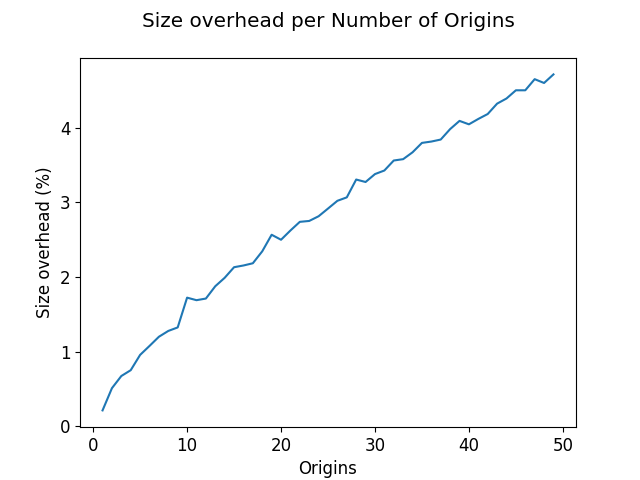
\includegraphics[width=0.48\textwidth]{experiments/origins.png}
        \caption{Origins}
        \label{fig:origin_ctx}
    \end{figure}

As Figure \ref{fig:origin_ctx} shows, the size overhead when 1 origin is used is less than 0.5\%
and about 4.7\% when 50 origins are used. This means that the compressed
response when CTX is used is expected to be 1.47x the unprotected compressed
response when 50 origins are used.

The second parameter, the total response size in bytes, affects the impact of
CTX on the compressed response.

In this case, we use 50 origins and consider 1\% of the total response to be
secret, equally distributed in all origins. The total response ranges from a
13KB to a 650KB web page.

Our experiments show that the increase in bytes that CTX adds is not
proportional to the increase of the total response size. This results in a
significant response size increase for small web pages, which becomes less
observable as the web page grows larger.

    \begin{figure}[thpb]
        \centering
            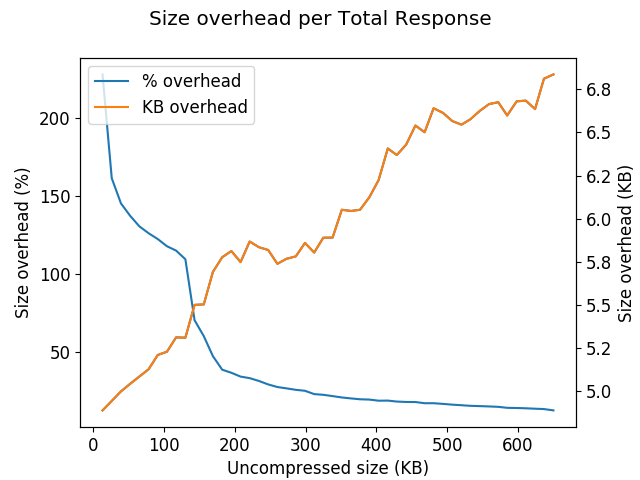
\includegraphics[width=0.48\textwidth]{experiments/total_response.png}
        \caption{Total response}
        \label{fig:total_response_ctx}
    \end{figure}

Figure \ref{fig:total_response_ctx} depicts the results of this experiment. A 13KB web page suffers a 5KB
CTX overhead, which corresponds to a 228\% increase in compressed response. On the
other hand, CTX will add only 7KB of compressed data for a 650KB web page, which
results in a 12\% increase. Disabling compression entirely would add overhead
that ranges from 500\% to 1000\% for the tested web pages.

The third parameter is the total amount of secrets in the response. In our
example we use a 650KB web page with 50 CTX origins. The secrets range from 1\%
up to 50\% of the web page, the rest being static data, and are evenly
distributed across origins.

    \begin{figure}[thpb]
        \centering
            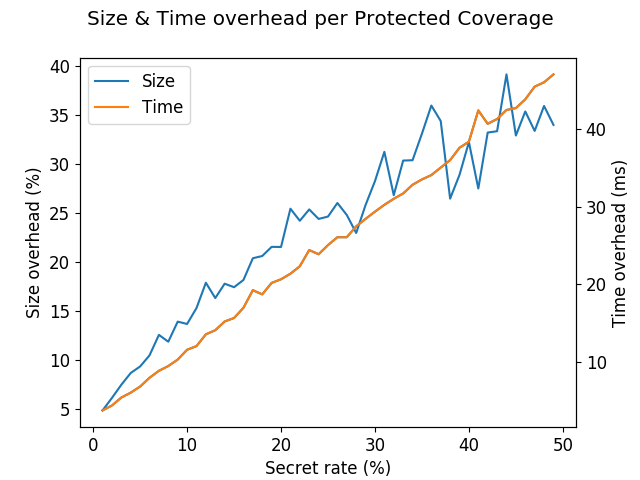
\includegraphics[width=0.48\textwidth]{experiments/response_secrets.png}
        \caption{Response secrets}
        \label{fig:response_secrets_ctx}
    \end{figure}

Figure \ref{fig:response_secrets_ctx} shows the results in this case. We find that protecting 1\% of the
tested web page results in less than 5\% size overhead, whereas protecting 50\% of
the page results in 35\%. This test also showed a noteworthy time increase in
execution time, where for 10\% secrets in the web page CTX adds 10ms of
execution time, while for 50\% it adds 47ms.

In comparison, disabling compression would again result in 976.8\% load overhead
and a network transmittion time overhead that, depending on the client's and the
server's network, may be several seconds.


In order to back our claim, we perform the following experiment. We choose a
fixed secret $s$, 100 characters long. We then choose the reflections $r_i,
i\in[0, 50]$, where $|r_i| = 50 + i*20$. For each $r_i$ we calculate the
length of separate compression using gzip $|gzip(s)||gzip(r_i)|$ and the length
of the compressed CTX'ed secret and reflection $|gzip(ctx(s), ctx(r_i))|$, where $s$
and $r_i$ belong to different origins.

The results are shown in figure \ref{fig:defense_experiment}. It can be seen
that the outputs of these two methods are linearly correlated, while also the
Pearson correlation coefficient of the two variables is 0.998712.

    \begin{figure}[thpb]
        \centering
            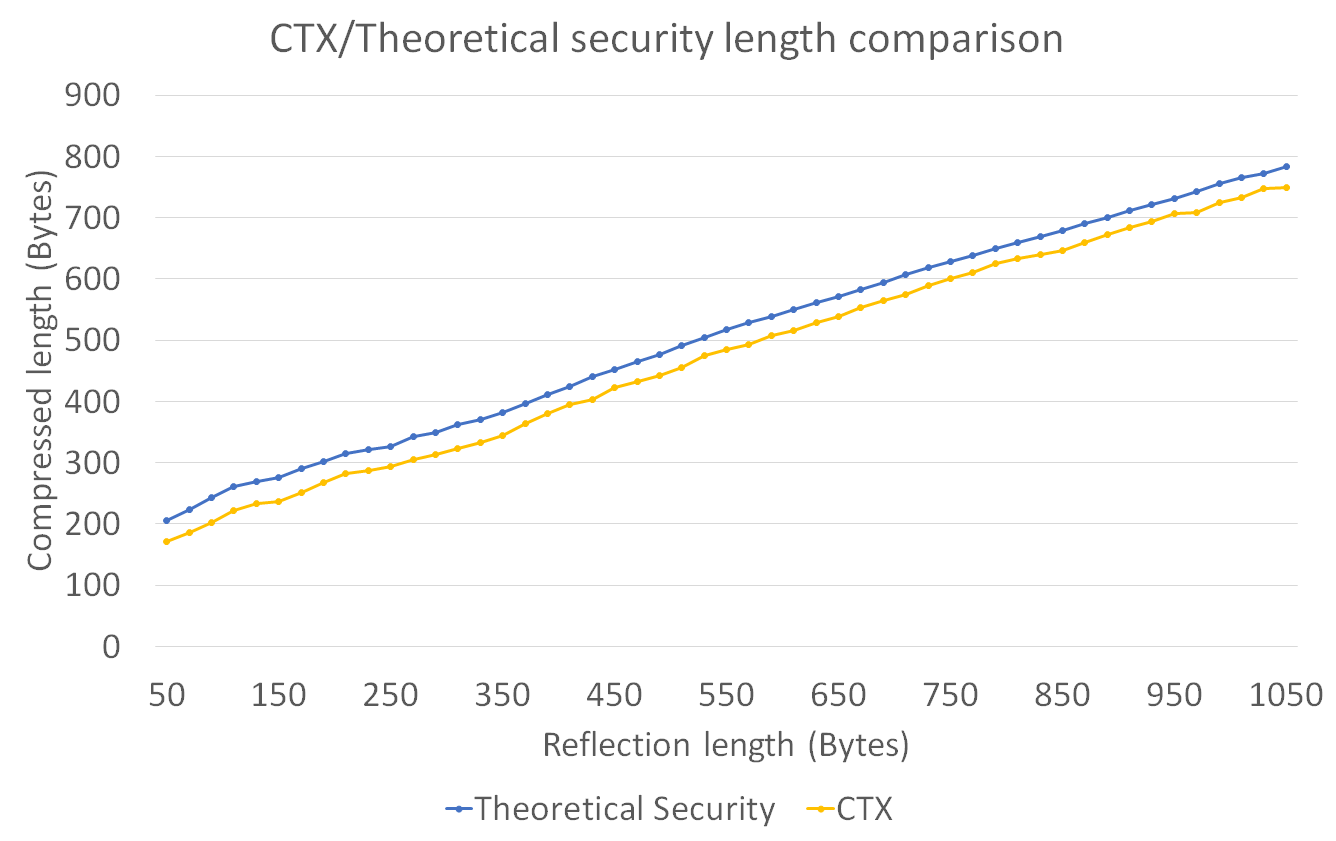
\includegraphics[width=0.48\textwidth]{defense_experiments/ctx_experiment.png}
        \caption{CTX/Theoretical security comparison}
        \label{fig:defense_experiment}
    \end{figure}


\bibliographystyle{abbrv}
\bibliography{citations}

\section{Full proofs}

\begin{lemma}[Semantic security]
\end{lemma}

\begin{proof}
    We will prove that if the scheme is not semantically secure, then it is
    necessarily not reflection secure. Assume that the scheme is not
    semantically secure. Then there will exist a PPT adversary $\mathcal{A}$
    such that for all PPT simulators $\mathcal{S}$ we have that $\mathcal{A}$
    has non-negligible advantage to $\mathcal{S}$ in the semantic security game.

    We will now construct an adversary $\mathcal{A'}$ for the reflection
    security game. $\mathcal{A'}$ operates as follows: It makes one query to
    the reflection oracle setting $r_0 = \epsilon$ and receives a response $c_0
    = K_k(s, r_0) = K_k(s) = c$. It then passes that $c$ to the semantic
    security adversary $\mathcal{A}$. It answers all encryption and decryption
    queries of the semantic security adversary by relaying them to its own
    encryption and decryption oracle. Finally, when the semantic security
    adversary outputs $y = y'$, this $y'$ is output by the reflection security
    adversary. Note that $\mathcal{A}$ cannot distinguish whether they are
    playing against the actual semantic security game or being simulated by the
    reflection security adversary, as their view is identical. Therefore:

    \begin{equation}
        Pr[Game_{REF-SEC}^{\mathcal{A'}} = 1] = Pr[Game_{SEM-SEC}^{\mathcal{A}} = 1]
    \end{equation}

    It remains to prove that $\mathcal{A'}$ has significant advantage against
    any reflection simulator $\mathcal{S'}$. Indeed let $\mathcal{S'}$ be any
    reflection game simulator. We will construct a simulator $\mathcal{S}$ for
    the semantic security game. Initially, the simulator $\mathcal{S}$ receives
    the length of the ciphertext $|c|$. They then simulate the reflection game
    simulator $\mathcal{S'}$ as follows. Upon receiving query $r_i$ from the
    reflection game simulator, they answer with $|c| + |r_i|$. When the
    reflection security adversary outputs $y' = y$, this $y$ is output by the
    semantic security simulator. We observe that the reflection game simulator
    $\mathcal{S'}$ cannot distinguish whether they are playing against the
    actual simulated reflection game or being simulated by the semantic
    security simulator. To see this, note that from the length preservation
    assumption we have that $|c| + |r_i| = |K(s, r_i)| = |K(s', r_i)| =
    |K(0^{|s|}, r_i)|$. Therefore:

    \begin{equation}
        Pr[Game_{SEM-SIM}^{\mathcal{S}} = 1] = Pr[Game_{REF-SIM}^{\mathcal{S'}} = 1]
    \end{equation}

    From the assumption that the scheme is not semantically insecure, we know
    that:

    \begin{align*}
        |Pr[Game_{SEM-SEC}^{\mathcal{A}} = 1] - Pr[Game_{SEM-SIM}^{\mathcal{S}} = 1]| =\\
        Adv_{\mathcal{A}, \mathcal{S}} = \text{non-negl}
    \end{align*}

    And therefore, replacing both probabilities with their equals:

    \begin{align*}
        |Pr[Game_{REF-SEC}^{\mathcal{A'}} = 1] -
        Pr[Game_{REF-SIM}^{\mathcal{S'}} = 1]| =\\
        Adv_{\mathcal{A'}, \mathcal{S'}} = \text{non-negl}
    \end{align*}
\end{proof}

\begin{lemma}[Good compression is detectable]
\end{lemma}

\begin{proof}
We model our plaintext input to the compression function as the usual pair $(s,
r)$ consisting of the secret string $s$ and reflection string $r$. When $(s, r)$
are encoded by a compression function $\mathcal{K}$ ideal under some plaintext
distribution $\bar{\mathcal{M}}$, a simple predicate allows the distinction
between two secrets $s_1$ and $s_2$ using a reflection pair $(r_1, r_2)$.  We
make the assumption that the resulting reflection pair $(r_1, r_2)$ is
efficiently computable.

\begin{align*}
    \Pr[r = r_1|s = s_1] < \Pr[r = r_2|s = s_1]&\land\\
    \Pr[r = r_1|s = s_2] > \Pr[r = r_2|s = s_2]&
\end{align*}

Using the fact that $\mathcal{K}$ is ideal with respect to this distribution,
we deduce that:

\begin{align*}
    |\mathcal{K}(s_1, r_1)| > |\mathcal{K}(s_1, r_2)|&\land\\
    |\mathcal{K}(s_2, r_1)| < |\mathcal{K}(s_2, r_2)|&
\end{align*}

We then define $Q(s)$ to be the predicate ``$s = s_1$". This partitions
$\mathcal{M}$ into the distributions $\mathcal{M}_Q$ and
$\mathcal{M}_{\lnot Q}$ both of which are non-empty, as $\mathcal{M}_Q$
contains $s_1$ and $\mathcal{M}_{\lnot Q}$ contains $s_2$. From the fact that
$Q$ is not trivial, we deduce that $\pi < 1$.

Observe, then, that letting $\bar{r} = (r_1, r_2)$ we obtain:

\begin{align*}
    \Pr[cpr^Q_{\mathcal{K}}(s_1, \bar{r}, \mathcal{K}, \mathcal{M})
    \land
    cpr^Q_{\mathcal{K}}(s_2, \bar{r}, \mathcal{K}, \mathcal{M})] = 1
\end{align*}

This completes the proof.

\end{proof}

\begin{lemma}[Compression attack]
\end{lemma}

\begin{proof}

Let $g$ be the boolean function $Q$ on the plaintext. Define the adversary
$\mathcal{A}$ as follows:

\begin{lstlisting}[texcl,mathescape,basicstyle=\small]
def $\mathcal{A}(1^\lambda)$:
    $(r_1, r_2) \leftarrow \mathcal{O}_R(1^\lambda)$

    $l_1 = |\text{Reflect}^{k}_s(r_1)|$
    $l_2 = |\text{Reflect}^{k}_s(r_2)|$

    if $l_1 < l_2$:
        return True
    else:
        return False
\end{lstlisting}

Let $\mathcal{S}$ be an arbitrary simulator. Then we have:
\begin{align*}
    \Pr[\text{Game}_{\text{REF-SIM}}^{\mathcal{SE},\mathcal{S}}
        (\lambda) = 1] &=\\
    \Pr_{x \leftarrow \mathcal{M}, b \leftarrow \mathcal{S}(1^\lambda)}
        [Q(x) = b]
\end{align*}

Letting the random variables $b$ and $x$:
\begin{align*}
    x &\leftarrow \mathcal{M}\\
    b &\leftarrow \mathcal{S}(1^\lambda)
\end{align*}

Due to the independence of the simulator's output with the choice of $x$ we have:
\begin{align*}
    Pr[b = Q(x)] &=\\
    Pr[\lnot b|\lnot Q(x)]Pr[\lnot Q(x)] + Pr[b|Q(x)]Pr[Q(x)] &=\\
    Pr[\lnot b]Pr[\lnot Q(x)] + Pr[b]Pr[Q(x)] &=\\
    (1 - Pr[b])(1 - Pr[Q]) + Pr[b]Pr[Q(x)] &=\\
    1 - Pr[Q(x)] - Pr[b] + 2Pr[b]Pr[Q(x)]
\end{align*}

For a given $\Pr[Q]$, this function is monotonic in $\Pr[b]$ and therefore has
potential extrema at $\Pr[b] = 0$ or $\Pr[b] = 1$, for which cases the function
takes the values $1 - \Pr[Q(x)]$ and $\Pr[Q(x)]$ respectively. Therefore, the
maximum $\Pr[b]$ of the simulator is:
\begin{equation*}
    \Pr[Q(x) = b] = max(\Pr[Q(x)], 1 - \Pr[Q(x)]) = \pi
\end{equation*}

And therefore:
\begin{align*}
    \forall \mathcal{S}:\\
    \Pr[
        \text{Game}_{\text{REF-SIM}}^{\mathcal{SE},\mathcal{S}}
        (\lambda) = 1
    ]
    \leq\\
    max(Pr[Q(x)], 1 - Pr[Q(x)])
\end{align*}

From the compression detectability of Q we know that:
\begin{align*}
    \exists \alpha \text{ non-negl}:\\
    \Pr_{s_1 \leftarrow \mathcal{M}_Q,
         s_2 \leftarrow \mathcal{M}_{\lnot Q}}
         [cpr^Q_{\kappa}(s_1, \overbar{r}) \land
          cpr^Q_{\kappa}(s_2, \overbar{r})]
    \geq\\
    \pi + \alpha(\lambda)
\end{align*}

Therefore:
\begin{align*}
    \Pr_{s_1 \leftarrow \mathcal{M}_Q}
         [cpr^Q_{\kappa}(s_1, \overbar{r})]
    \geq
    \pi + \alpha(\lambda) \land\\
    \Pr_{s_2 \leftarrow \mathcal{M}_{\lnot Q}}
         [cpr^Q_{\kappa}(s_2, \overbar{r})]
    \geq
    \pi + \alpha(\lambda)
\end{align*}

And so:
\begin{align*}
    \Pr_{s \leftarrow \mathcal{M}}
         [cpr^Q_{\kappa}(s, \overbar{r})]
    =\\
    \Pr[cpr^Q_{\kappa}(s, \overbar{r})|Q(s)]\Pr[Q(s)]
    +\\
    \Pr[cpr^Q_{\kappa}(s, \overbar{r})|\lnot Q(s)]\Pr[\lnot Q(s)]
    \geq\\
    (\pi + \alpha(\lambda))(\Pr[Q(s)] + (1 - \Pr[Q(s)))
    =\\
    \pi + \alpha(\lambda)
\end{align*}

Let us now examine the event of $\mathcal{A}$ being successful, denoted Succ,
when $cpr^Q_{\kappa}(s, \overbar{r})$. Assuming $Q(s)$:
\begin{align*}
    \Pr[|\mathcal{K}(s, r_1)| < |\mathcal{K}(s, r_2)||Q(s)]
    = \pi + \alpha(\lambda)
\end{align*}

And from the strict length monotonicity of $\textrm{Enc}$ it follows that:
\begin{align*}
    \Pr[&|\textrm{Enc}(\mathcal{K}(s, r_1))| <\\&|\textrm{Enc}(\mathcal{K}(s, r_2))||Q(s)]
        \geq \pi + \alpha(\lambda)\\
    \Rightarrow \Pr[&
        |\text{Reflect}^{k}_s(r_1)|
        <
        |\text{Reflect}^{k}_s(r_2)||Q(s)
    ]
        \geq \pi + \alpha(\lambda)\\
    \Rightarrow \Pr[&l_1 < l_2|Q(s)]
        \geq \pi + \alpha(\lambda)\\
    \Rightarrow \Pr[&\text{Succ}|Q(s)]
        \geq \pi + \alpha(\lambda)\\
\end{align*}

The case for $\lnot Q(s)$ is the same, but with a different inequality direction:
\begin{align*}
    \Pr[|\mathcal{K}(s, r_1)| > |\mathcal{K}(s, r_2)||\lnot Q(s)]
        \geq\\
        \pi + \alpha(\lambda)\\
    \Rightarrow \Pr[\text{Succ}|\lnot Q(s)] \geq\\
    \pi + \alpha(\lambda)\\
\end{align*}

And so the probability of success is given:
\begin{align*}
    \Pr[\text{Succ}] =\\
    \Pr[\text{Succ}|Q(s)]\Pr[Q(s)]
    +
    \Pr[\text{Succ}|\lnot Q(s)]\Pr[\lnot Q(s)] \geq\\
    \pi + \alpha(\lambda)
\end{align*}

Therefore,
\begin{align*}
    \forall PPT \mathcal{S}:
    \text{Adv}_{\mathcal{SE}(\textrm{Enc}, \textrm{Com}), \mathcal{A}, \mathcal{S}}
        (1^\lambda)
    \geq\\
    |\pi + \alpha(\lambda) - \pi| = \alpha(\lambda)
\end{align*}

Which is non-negligible.

\end{proof}

\begin{lemma}[Amplification]
\end{lemma}

\begin{proof}

From the fact that $Q$ is compression-detectable and from the Compression Attack Theorem, we have that:
\begin{align*}
    \Pr_{s \leftarrow \mathcal{M}}
         [cpr^Q_{\kappa}(s, \overbar{r})]
    =\\
    \pi + \alpha(\lambda)
\end{align*}

Some elements $s \in \mathcal{M}$ allow for better compression detectability than others under the fixed
reflection vector $\overbar{r}$. Call these elements \textit{amplifiable} and define predicate:
\begin{align*}
    Amp(s) \defeq
    \Pr[cpr^Q_{\kappa}
     (s, \overbar{r})]
    \geq
    \frac{1}{2} + \frac{\alpha(\lambda)}{2}
\end{align*}

We will now obtain a lower bound on the probability of an element being amplifiable.

Let:

% B derivation: (where \beta(\lambda) = \alpha(\lambda) / 2)
% B + (\frac{1}{2} + \alpha(\lambda)/2)(1 - B) = \pi + \alpha(\lambda)
% B + \frac{1}{2} + \alpha(\lambda)/2 - B(\frac{1}{2} + \beta(\lambda)) = \pi + \alpha(\lambda)
% \frac{1}{2} + \beta(\lambda) + B(\frac{1}{2} - \beta(\lambda)) = \pi + \alpha(\lambda)
% B(\frac{1}{2} - \beta(\lambda)) = \pi + \alpha(\lambda) - \frac{1}{2} - \beta(\lambda)
% B = (\pi + \alpha(\lambda) - \frac{1}{2} - \beta(\lambda)) / (\frac{1}{2} - \beta(\lambda))
% B = (\pi + \alpha(\lambda) - \frac{1}{2} - \frac{\alpha(\lambda)}{2}) / (\frac{1}{2} - \frac{\alpha(\lambda)}{2})
% B = (\pi - \frac{1}{2} + \frac{\alpha(\lambda)}{2}) / (\frac{1}{2} - \frac{\alpha(\lambda)}{2})
% B = \pi / (\frac{1}{2} - \frac{\alpha(\lambda)}{2}) - (\frac{1}{2} - \frac{\alpha(\lambda)}{2}) / (\frac{1}{2} - \frac{\alpha(\lambda)}{2})
% B = \pi / (\frac{1}{2} - \frac{\alpha(\lambda)}{2}) - 1
\begin{align*}
    B = \frac{\pi}{\frac{1}{2} - \frac{\alpha(\lambda)}{2}} - 1
\end{align*}

$B$ is non-negligible in $\lambda$.

Assume, for the sake of contradiction, that:
\begin{align*}
    \Pr_{s \leftarrow \mathcal{M}}
    [Amp(s)] < B
\end{align*}

Then we have:
\begin{align*}
    \Pr_{s \leftarrow \mathcal{M}}
         [cpr^Q_{\kappa}(s, \overbar{r})]
    =\\
    \Pr_{s \leftarrow \mathcal{M}}
         [cpr^Q_{\kappa}(s, \overbar{r})|Amp(s)]\Pr[Amp(s)]
    +\\
    \Pr_{s \leftarrow \mathcal{M}}
         [cpr^Q_{\kappa}(s, \overbar{r})|\lnot Amp(s)]\Pr[\lnot Amp(s)]
    <\\
    B + (\frac{1}{2} + \frac{\alpha}{2})(1 - B)
\end{align*}

But then:
\begin{align*}
    B + (\frac{1}{2} + \frac{\alpha(\lambda)}{2})(1 - B) =
    \pi + \alpha(\lambda)
\end{align*}

And this contradicts the assumption that $Q$ is compression-detectable. Therefore:
\begin{align*}
    \Pr_{s \leftarrow \mathcal{M}}
    [Amp(s)] \geq B
\end{align*}

It remains to show that the advantage of the adversary can be
arbitrarily large, i.e. that for some negligible $C$ we have:
\begin{align*}
    \text{Adv}_{\mathcal{SE}(\textrm{Enc}, \textrm{Com}), \mathcal{A}, \mathcal{S}_{Amp}}
    (1^\lambda) = 1 - \pi - C
\end{align*}

Indeed, observe that the amplifying adversary performs a repeated Bernoulli
trial with $k$ repetitions and extracts a majority. Let $X$ be the number of
repetitions that are successful for the adversary. $X$ is defined:
\begin{align*}
    X \defeq |\{ i: cpr^Q_{\kappa}(s, \overbar{r}) \}|
\end{align*}

$X$ follows the binomial distribution, and therefore its expected value is:
\begin{align*}
    E[X] = \frac{k}{2} + \frac{\alpha k}{2}
\end{align*}

Let Succ denote the event of the amplified adversary succeeding. Then Succ
is equivalent to $X > \frac{k}{2}$.

Because $\alpha$ is non-negligible and due to the tail bounds of the binomial
distribution, we have:
\begin{align*}
    Pr[Succ] = 1 - C(k)
\end{align*}

Where $C$ is a negligible function.
\end{proof}

\begin{lemma}[Reflection-independent security]
    Let $E$ be a length-preserving semantically secure encryption schema and
    $Com$ be any function. Then $E(s)$ is reflection secure.
\end{lemma}

\begin{proof}
    Let $\mathcal{A}$ be a reflection security adversary for $E(s)$. We will
    construct a semantic security adversary $\mathcal{A'}$ for $E$. Our semantic
    security adversary will break semantic security for \textit{multiple
    messages}. Let $\mathcal{M}$ be the distribution that $\mathcal{A}$
    attacks. Because $\mathcal{A}$ is a probabilistic polynomial-time
    adversary, there is a polynomial bound $t(\lambda)$ for its execution time.
    The number of reflection queries conducted by $\mathcal{A}$ is then also
    bound by $t(\lambda)$.

    Define $\mathcal{M'}$ by the following procedure: First, $s$ is chosen
    out of the distribution $\mathcal{M}$. Then that same $s$ is repeated
    $t(\lambda)$ times to obtain the vector of plaintexts $\overbar{s}$.

    Upon execution, $\mathcal{A'}$ receives from its challenger the encrypted
    vector $\overbar{c}$ where the same plaintext has been independently
    encrypted $t(\lambda)$ times.
    $\mathcal{A'}$ answers encryption and decryption queries of $\mathcal{A}$
    by forwarding them to its own encryption and
    decryption oracles. For reflection queries, because the schema trivially
    ignores $r$ since $E(s)$ is independent of $r$, the semantic security
    adversary is able to answer each query $r_i$ with $c_i$.

    Clearly, the view of the simulated reflection adversary is the same as if
    it were run in an actual reflection game. Therefore we have:

    \begin{align*}
        Pr[\text{Game}_{\text{REF-SEC}}^{\mathcal{A}}(1^{\lambda})
        = 1]
        =
        Pr[\text{Game}_{\text{SEM-SEC}}^{\mathcal{A'}}(1^{\lambda})
        = 1]
    \end{align*}

    We now prove that the adversary $\mathcal{A'}$ obtains a non-negligible gap
    against any semantic security simulator $\mathcal{S'}$. Indeed let
    $\mathcal{S'}$ be any semantic security simulator. We will construct a
    reflection security simulator $\mathcal{S}$. $\mathcal{S}$ works as
    follows: It obtains $|Com(s)|$ from its challenger which it ignores. It
    then issues a single reflection query $r_1 = \epsilon$, to which the
    challenger responds with $c = E(s')$. But $|c| = |E(s')| = |s'| =
    |0^{|s|}| = |s| = |E(s)| = |c|$ due to length preservation. This $|c|$ is
    then used to start the semantic security simulator.

    The view of the simulated semantic simulator is the same as if it were run
    in an actual semantic simulation game. Therefore we have:

    \begin{align*}
        Pr[\text{Game}_{\text{REF-SIM}}^{\mathcal{S}}(1^{\lambda})
        = 1]
        =
        Pr[\text{Game}_{\text{SEM-SIM}}^{\mathcal{S'}}(1^{\lambda})
        = 1]
    \end{align*}

    Because there exists a non-negligible advantage between $\mathcal{A}$ and
    any simulator $\mathcal{S}$, this gap will also exist between the
    constructed simulator $\mathcal{S}$. Therefore, we have:

    \begin{align*}
        \text{non-negl} = \text{Adv}_{\text{REF} \mathcal{A}, \mathcal{S}}\\
        =
        Pr[\text{Game}_{\text{REF-SEC}}^{\mathcal{A}}
        = 1] -
        Pr[\text{Game}_{\text{REF-SIM}}^{\mathcal{S}}
        = 1]\\
        =
        Pr[\text{Game}_{\text{SEM-SEC}}^{\mathcal{A'}}
        = 1]
        -
        Pr[\text{Game}_{\text{SEM-SIM}}^{\mathcal{S'}}
        = 1]\\
        =
        \text{Adv}_{\text{SEM} \mathcal{A'}, \mathcal{S'}}
    \end{align*}

    For clarity, we have omitted the security parameters from the games.
    This completes the proof.
\end{proof}

\begin{lemma}
    Under the above assumptions, $E(s) || r$ is reflection secure.
\end{lemma}

\begin{proof}
    The construction is identical to the previous proof. However, the
    reflection queries of the reflection adversary $\mathcal{A}$ must be
    answered correctly. As $r_i$ is known to the semantic security adversary,
    this can be done in the obvious way by setting $c_i' = c_i || r_i$.

    The reflection security simulator is not affected, as it receives $|c| =
    |Enc(s) || \epsilon| = |Enc(s)|$.
\end{proof}

\begin{lemma}
    Under the above assumptions and letting $Com$ be a deterministic
    efficiently computable function, $E(s)$ $||$ $Com(r)$ is reflection secure.
\end{lemma}

\begin{proof}
    The construction is the same as before. Because the semantic security
    adversary has access to the $Com$ function, it can calculcate $Com(r_i)$
    upon receiving the query $r_i$. Then setting $c_i = E(s) || Com(r_i)$ it
    responds as usual.

    The reflection simulator on the other hand will be affected by this
    construction. Indeed $|c| = |E(s') || Com(\epsilon)|$. However,
    $|Com(\epsilon)|$ can be computed by the simulator, and therefore the value
    given to the semantic simulator can be obtained as $|c'| = |E(s)| = |E(s')|
    = |c| - |Com(\epsilon)|$.
\end{proof}

\begin{lemma}
    Under the above assumptions and additionally requiring that $Com$ is a
    bijection which is also efficiently reversible, $E(Com(s))$ is reflection secure.
\end{lemma}

\begin{proof}
    This construction is slightly more complicated. Assuming $\mathcal{A}$ is a
    reflection-security adversary which works against the distribution
    $\mathcal{M}$ we will construct a multiple messages semantic security
    adversary as before. However, the distribution $\mathcal{M'}$ will now be
    obtained by the following procedure: Initially, $s$ is chosen out of
    $\mathcal{M}$. Then $Com(s)$ is calculated. This value is then repeated
    $t(\lambda)$ times. Our semantic security adversary will work against
    $\mathcal{M'}$.

    When the challenger produces the encrypted vector $\overbar{c}$, it will
    contain $t(\lambda)$ encryptions of the plaintext $Com(s)$. These can
    readily now be passed to the reflection adversary as reflection query
    responses as before.

    The reflection security simulator now makes use of the $|Com(s)|$ input,
    which it uses to start up the semantic security simulator.

    We now argue that the advantage obtained pertains to a valid predicate on
    the compressed plaintexts space. Indeed, without loss of generality assume
    that $g$ is a predicate. Then $g$ partitions the plaintext space into two
    partitions. Due to $Com$ being a bijection, these partitions are preserved
    after compression and the plaintext predicate $g$ is isomorphic to a
    compressed text predicate $g'$. Therefore, the semantic security adversary
    is able to obtain a non-negligible advantage for a different predicate.
\end{proof}

\begin{lemma}
    Under the above assumptions, $E(Com(s)) || r)$, \break$E(Com(s)) || E(r))$, and
    $E(Com(s)) || E(Com(r))$ are all reflection secure.
\end{lemma}

\begin{proof}
    The proofs for the above schemas can be combined in the obvious way to
    obtain the result needed.
\end{proof}

\begin{lemma}
    Under the above assumptions, $E(s || r)$ is reflection secure.
\end{lemma}

\begin{proof}
    We provide a sketch of this proof.

    To obtain this proof, we construct a semantic security adversary which
    works against a distribution $\mathcal{M'}$ defined as follows. First, $s$
    is chosen out of $\mathcal{M}$. Because the reflection security adversary
    is bounded in time by $t(\lambda)$, therefore each of the reflection
    queries $r_i$ must be $|r_i| < t(\lambda)$. The distribution $\mathcal{M'}$
    then will contain $t(\lambda)$ different vectors, each of dimension
    $t(\lambda)$. We require that the $j$-th $t$-dimensional vector contains
    the same secret text $s$ and an independently chosen reflection text $r$
    with $|r| = j$.

    Then the semantic security adversary $\mathcal{A'}$ works as follows: Upon
    receiving the reflection query $r_i$ from the reflection adversary, it
    responds with a fresh element from the $i$-th vector, which contains the
    encryption of an incorrect reflection string chosen uniformly at random. We
    call these \textit{mock} reflections, and notice that the mock reflection
    has the same length as the actual reflection query.

    We now argue that either this semantic security adversary is able to obtain
    a valid predicate for $s$, or that we have obtained a distinguisher for the
    value $r$.

    To do this, invoke a hybrid argument on the sequence of adversaries $B_i$
    such that the $i$-th adversary works as follows: It responds to the
    reflection queries $r_1, r_2, \cdots, r_i$ as $\mathcal{A'}$ would,
    using the mock reflections, but responds to the queries $r_{i+1},
    \cdots, r_{t(\lambda)}$ using the correct reflections. Clearly,
    $\mathcal{A'} = B_{t(\lambda)}$. If for all $j$ we have that $B_j$'s output
    is computationally indistinguishable from $B_{j+1}$'s output, we are done,
    since this would allow the construction of $\mathcal{A'}$ that obtains a
    non-negligible advantage. However, if for some $j$ we have that $B_j$'s
    output is computationally distinguishable from $B_{j+1}$, then this
    directly allows the construction of a semantic security adversary which is
    able to distinguish between different $r$ values. The intuition behind this
    is that since the mock and actual reflection queries have the same length,
    the assumption of semantic security should not allow the reflection
    adversary to tell apart the two reflection responses.
\end{proof}

\begin{lemma}
    Under the above assumptions, $E(Com(s)$ $||$ $Com(r))$ is reflection secure.
\end{lemma}

\begin{proof}
    The above lemma follows directly from the fact that $E(s || r)$ is
    reflection secure using the techniques previously used to obtain the
    reflection security of $E(Com(s))$ and $E(Com(s))$ $||$ $E(Com(r))$. For the
    compression of the secret, the key intuition is that the reflection
    adversary has access to $|Com(s)|$, that the predicate attacked will be an
    isomorphic predicate on compression space instead of plaintext space, and
    that the distribution attacked will be the compression distribution instead
    of the plaintext distribution. This is readily obtained from the fact that
    $Com$ is a bijection. For the $Com(r)$ portion, the only
    requirement is that the compression function is accessible to both the
    semantic security adversary as well as the reflection security simulator,
    which is true under the assumption that $Com(r)$ is deterministic.
\end{proof}

\section{Related work}\label{sec:related}

\subsection{Compression attacks in literature}

The compression side-channel attack technique was first studied by Kelsey
\cite{kelsey2002compression} in 2002.
Kelley and Tamassia\cite{kelley2014secure} discuss the notion of \textit{entropy-restricted} semantic
security. However, this only models the case where two secrets compress to the same
length, making it difficult to capture practical techniques used in attacks
such as BREACH.

Alawatugoda et al. \cite{alawatugoda2015protecting} introduce a model for \textit{Cookie recovery},
\textit{Random cookie indistinguishability}, and \textit{Chosen cookie indistinguishability}.
Nevertheless, their security models are limited in classes of rendering functions
that are very specific. In their models, the attacker is able to directly influence
the output of the rendering function through concatenation. More information on
rendering functions is provided in section \ref{subsec:terms}.

\subsection{Defenses}

Literature includes many proposed defenses for side-channel compression attacks
and especially BREACH, some of which are explored in the following sections.

\subsubsection{Disabling compression}\label{subsec:disablecom}
Compression is the basic assumption for the compression detectability. Disabling
compression would break the adaptive reflection game.

However, this is not a viable solution. Disabling compression results in a
performance penalty that outweighs the benefits of the defense.

\subsubsection{SameSite cookies}\label{subsec:samesite}
SameSite cookies \cite{mwest2015firstparty} is a proposed draft for enhancing
web security. The main puprose of this technique is to mitigate cross-site
request forgery attacks, although it also mitigates other kinds of cross-origin
leakages.

This policy introduces a new attribute for web cookies that web servers may
opt-in. This attribute states that cookies may only be included in a
``first-party" context, i.e. in same origin requests.

However, the current BREACH application depends on cross-origin requests in
order to call the reflection oracle. Enabling SameSite cookies would result in
the elimination of this reflection oracle of the Reflection-Security Game.

\subsubsection{Masking secrets}\label{subsec:masking}
Masking is a method of hiding secrets' properties.

A mask is a bitstream equal in size with the secret. The masked text contains
the result of the XOR operation between the secret and the mask. The masked
secret is then concatenated with the mask that was used. The secret can be
obtained by applying XOR between the masked secret and the mask.

A new mask is used for each request. That way, the secret's content is secured
against instances of the attack that require at least two calls to the
reflection oracle.

However, masking doubles the size of the protected secret. Furthermore, the mask
is random, and so is the masked secret, so the compression performance is poor.
Therefore, masking should be applied on high value secrets only, in order to
avoid significant performance penalties.

Masking is a method used by Facebook \cite{facebookbreach} in order to protect CSRF tokens
against BREACH attacks.

\section*{Appendix C: Experiments}

\subsection{Idealness experiments}

We now turn our attention to two specific compression functions, the
LZ77 and Huffman function. These two compression functions are of
interest for two reasons. First, they are representative of the way
typical lossless compression functions work internally, by taking
advantage of letter frequencies (Huffman) or letter-sequence
repetitions (LZ77). Second, they are the ones almost exclusively used in
practice. The DEFLATE algorithm \cite{deutsch1996deflate}, which is a composition of LZ77 and
Huffman, is the algorithm used in gzip, which is prevalent on the
modern web. In 2016, 98.85\% of websites that enabled compression used
some form of gzip. We argue that both LZ77 and Huffman are nearly
ideal compression functions. The complexity of the Huffman and
especially the LZ77 algorithms arises from many intricate technical
details, such as, for instance, the sliding window size of LZ77. These
details make it impractical to deal with these functions in analytical
proofs.

We support our idealness claims in an experimental manner. Our experiment
measured the compression performance of the Huffman and an ideal function on a
text of English literature\footnote{The screenplay of the movie "The Social
Network".}. First, we calculated the occurences of each character (letters and
digits) in the text. Second, we generated the Huffman
table for this text and the table of an ideal function based on the character
frequencies. Each character is represented by a bitstream in both tables. Figure
\ref{fig:huffman_idealness} depicts the length of the bitstreams of characters
in descending order of occurencies for both the ideal and the Huffman functions.

    \begin{figure}[thpb]
        \centering
            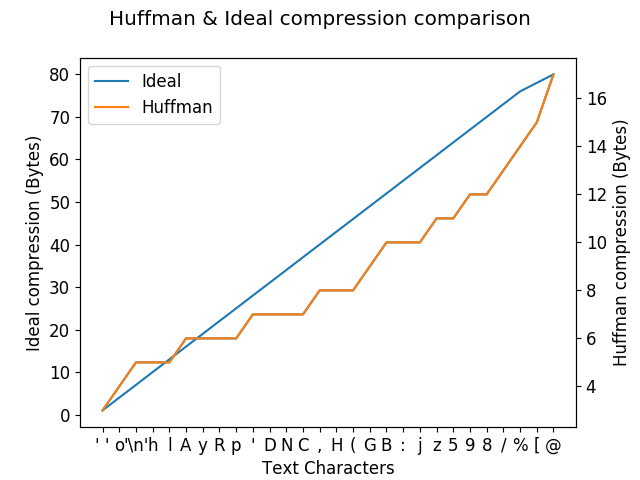
\includegraphics[width=0.48\textwidth]{idealness_experiments/huffman_idealness.png}
        \caption{Huffman-ideal compression comparison}
        \label{fig:huffman_idealness}
    \end{figure}



\end{document}
